% Options for packages loaded elsewhere
\PassOptionsToPackage{unicode}{hyperref}
\PassOptionsToPackage{hyphens}{url}
%
\documentclass[
]{article}
\usepackage{amsmath,amssymb}
\usepackage{lmodern}
\usepackage{iftex}
\ifPDFTeX
  \usepackage[T1]{fontenc}
  \usepackage[utf8]{inputenc}
  \usepackage{textcomp} % provide euro and other symbols
\else % if luatex or xetex
  \usepackage{unicode-math}
  \defaultfontfeatures{Scale=MatchLowercase}
  \defaultfontfeatures[\rmfamily]{Ligatures=TeX,Scale=1}
\fi
% Use upquote if available, for straight quotes in verbatim environments
\IfFileExists{upquote.sty}{\usepackage{upquote}}{}
\IfFileExists{microtype.sty}{% use microtype if available
  \usepackage[]{microtype}
  \UseMicrotypeSet[protrusion]{basicmath} % disable protrusion for tt fonts
}{}
\makeatletter
\@ifundefined{KOMAClassName}{% if non-KOMA class
  \IfFileExists{parskip.sty}{%
    \usepackage{parskip}
  }{% else
    \setlength{\parindent}{0pt}
    \setlength{\parskip}{6pt plus 2pt minus 1pt}}
}{% if KOMA class
  \KOMAoptions{parskip=half}}
\makeatother
\usepackage{xcolor}
\usepackage[top=2cm,bottom=2cm]{geometry}
\usepackage{color}
\usepackage{fancyvrb}
\newcommand{\VerbBar}{|}
\newcommand{\VERB}{\Verb[commandchars=\\\{\}]}
\DefineVerbatimEnvironment{Highlighting}{Verbatim}{commandchars=\\\{\}}
% Add ',fontsize=\small' for more characters per line
\usepackage{framed}
\definecolor{shadecolor}{RGB}{248,248,248}
\newenvironment{Shaded}{\begin{snugshade}}{\end{snugshade}}
\newcommand{\AlertTok}[1]{\textcolor[rgb]{0.94,0.16,0.16}{#1}}
\newcommand{\AnnotationTok}[1]{\textcolor[rgb]{0.56,0.35,0.01}{\textbf{\textit{#1}}}}
\newcommand{\AttributeTok}[1]{\textcolor[rgb]{0.77,0.63,0.00}{#1}}
\newcommand{\BaseNTok}[1]{\textcolor[rgb]{0.00,0.00,0.81}{#1}}
\newcommand{\BuiltInTok}[1]{#1}
\newcommand{\CharTok}[1]{\textcolor[rgb]{0.31,0.60,0.02}{#1}}
\newcommand{\CommentTok}[1]{\textcolor[rgb]{0.56,0.35,0.01}{\textit{#1}}}
\newcommand{\CommentVarTok}[1]{\textcolor[rgb]{0.56,0.35,0.01}{\textbf{\textit{#1}}}}
\newcommand{\ConstantTok}[1]{\textcolor[rgb]{0.00,0.00,0.00}{#1}}
\newcommand{\ControlFlowTok}[1]{\textcolor[rgb]{0.13,0.29,0.53}{\textbf{#1}}}
\newcommand{\DataTypeTok}[1]{\textcolor[rgb]{0.13,0.29,0.53}{#1}}
\newcommand{\DecValTok}[1]{\textcolor[rgb]{0.00,0.00,0.81}{#1}}
\newcommand{\DocumentationTok}[1]{\textcolor[rgb]{0.56,0.35,0.01}{\textbf{\textit{#1}}}}
\newcommand{\ErrorTok}[1]{\textcolor[rgb]{0.64,0.00,0.00}{\textbf{#1}}}
\newcommand{\ExtensionTok}[1]{#1}
\newcommand{\FloatTok}[1]{\textcolor[rgb]{0.00,0.00,0.81}{#1}}
\newcommand{\FunctionTok}[1]{\textcolor[rgb]{0.00,0.00,0.00}{#1}}
\newcommand{\ImportTok}[1]{#1}
\newcommand{\InformationTok}[1]{\textcolor[rgb]{0.56,0.35,0.01}{\textbf{\textit{#1}}}}
\newcommand{\KeywordTok}[1]{\textcolor[rgb]{0.13,0.29,0.53}{\textbf{#1}}}
\newcommand{\NormalTok}[1]{#1}
\newcommand{\OperatorTok}[1]{\textcolor[rgb]{0.81,0.36,0.00}{\textbf{#1}}}
\newcommand{\OtherTok}[1]{\textcolor[rgb]{0.56,0.35,0.01}{#1}}
\newcommand{\PreprocessorTok}[1]{\textcolor[rgb]{0.56,0.35,0.01}{\textit{#1}}}
\newcommand{\RegionMarkerTok}[1]{#1}
\newcommand{\SpecialCharTok}[1]{\textcolor[rgb]{0.00,0.00,0.00}{#1}}
\newcommand{\SpecialStringTok}[1]{\textcolor[rgb]{0.31,0.60,0.02}{#1}}
\newcommand{\StringTok}[1]{\textcolor[rgb]{0.31,0.60,0.02}{#1}}
\newcommand{\VariableTok}[1]{\textcolor[rgb]{0.00,0.00,0.00}{#1}}
\newcommand{\VerbatimStringTok}[1]{\textcolor[rgb]{0.31,0.60,0.02}{#1}}
\newcommand{\WarningTok}[1]{\textcolor[rgb]{0.56,0.35,0.01}{\textbf{\textit{#1}}}}
\usepackage{longtable,booktabs,array}
\usepackage{calc} % for calculating minipage widths
% Correct order of tables after \paragraph or \subparagraph
\usepackage{etoolbox}
\makeatletter
\patchcmd\longtable{\par}{\if@noskipsec\mbox{}\fi\par}{}{}
\makeatother
% Allow footnotes in longtable head/foot
\IfFileExists{footnotehyper.sty}{\usepackage{footnotehyper}}{\usepackage{footnote}}
\makesavenoteenv{longtable}
\usepackage{graphicx}
\makeatletter
\def\maxwidth{\ifdim\Gin@nat@width>\linewidth\linewidth\else\Gin@nat@width\fi}
\def\maxheight{\ifdim\Gin@nat@height>\textheight\textheight\else\Gin@nat@height\fi}
\makeatother
% Scale images if necessary, so that they will not overflow the page
% margins by default, and it is still possible to overwrite the defaults
% using explicit options in \includegraphics[width, height, ...]{}
\setkeys{Gin}{width=\maxwidth,height=\maxheight,keepaspectratio}
% Set default figure placement to htbp
\makeatletter
\def\fps@figure{htbp}
\makeatother
\setlength{\emergencystretch}{3em} % prevent overfull lines
\providecommand{\tightlist}{%
  \setlength{\itemsep}{0pt}\setlength{\parskip}{0pt}}
\setcounter{secnumdepth}{-\maxdimen} % remove section numbering
\setlength{\parskip}{1ex plus 0.5ex minus 0.5ex}
\ifLuaTeX
  \usepackage{selnolig}  % disable illegal ligatures
\fi
\IfFileExists{bookmark.sty}{\usepackage{bookmark}}{\usepackage{hyperref}}
\IfFileExists{xurl.sty}{\usepackage{xurl}}{} % add URL line breaks if available
\urlstyle{same} % disable monospaced font for URLs
\hypersetup{
  pdftitle={A4 - Análisis estadístico avanzado},
  pdfauthor={Leroy Deniz},
  hidelinks,
  pdfcreator={LaTeX via pandoc}}

\title{A4 - Análisis estadístico avanzado}
\usepackage{etoolbox}
\makeatletter
\providecommand{\subtitle}[1]{% add subtitle to \maketitle
  \apptocmd{\@title}{\par {\large #1 \par}}{}{}
}
\makeatother
\subtitle{Estadística Avanzada}
\author{Leroy Deniz}
\date{Actualizado: 26 December, 2022}

\begin{document}
\maketitle

\tableofcontents

\newpage

\hypertarget{contexto}{%
\section{0 Contexto}\label{contexto}}

\begin{center}\rule{0.5\linewidth}{0.5pt}\end{center}

\hypertarget{importaciuxf3n-de-libreruxedas}{%
\subsection{0.1 Importación de
librerías}\label{importaciuxf3n-de-libreruxedas}}

\begin{Shaded}
\begin{Highlighting}[]
\FunctionTok{library}\NormalTok{(ggplot2)}
\FunctionTok{library}\NormalTok{(tidyverse)}
\FunctionTok{library}\NormalTok{(reshape2)}
\FunctionTok{library}\NormalTok{(stats)}
\FunctionTok{library}\NormalTok{(dplyr)}
\end{Highlighting}
\end{Shaded}

\hypertarget{funciones-auxiliares}{%
\subsection{0.2 Funciones auxiliares}\label{funciones-auxiliares}}

\begin{Shaded}
\begin{Highlighting}[]
\CommentTok{\# Función para mostrar información en vertical}
\NormalTok{vertical }\OtherTok{\textless{}{-}} \ControlFlowTok{function}\NormalTok{(tbl) \{}
    \FunctionTok{t}\NormalTok{(}\FunctionTok{t}\NormalTok{(tbl))}
\NormalTok{\}}
\end{Highlighting}
\end{Shaded}

\hypertarget{configuraciones}{%
\subsection{0.3 Configuraciones}\label{configuraciones}}

\begin{Shaded}
\begin{Highlighting}[]
\FunctionTok{options}\NormalTok{(}\AttributeTok{dplyr.summarise.inform =} \ConstantTok{FALSE}\NormalTok{)}
\end{Highlighting}
\end{Shaded}

\newpage

\hypertarget{preprocesado}{%
\section{1 Preprocesado}\label{preprocesado}}

\begin{center}\rule{0.5\linewidth}{0.5pt}\end{center}

\hypertarget{lectura-del-fichero}{%
\subsection{1.1 Lectura del fichero}\label{lectura-del-fichero}}

\begin{Shaded}
\begin{Highlighting}[]
\NormalTok{df }\OtherTok{\textless{}{-}} \FunctionTok{read.csv}\NormalTok{(}\StringTok{"Fumadores.csv"}\NormalTok{, }\AttributeTok{sep =} \StringTok{";"}\NormalTok{, }\AttributeTok{dec =} \StringTok{"."}\NormalTok{)}
\end{Highlighting}
\end{Shaded}

\vspace{0.3cm}

Muestra del dataset generado a raíz de la lectura:

\vspace{0.3cm}

\begin{Shaded}
\begin{Highlighting}[]
\FunctionTok{head}\NormalTok{(df)}
\end{Highlighting}
\end{Shaded}

\begin{verbatim}
##         AE Tipo genero edad
## 1 1.871878   NF      M   54
## 2  1.91312   NF      F   60
## 3  2.58114   NF      M   40
## 4  2.17827   NF      F   55
## 5 1.707732   NF      F   59
## 6 1.561215   NF      F   63
\end{verbatim}

\hypertarget{consulta-de-tipos-y-transformaciones}{%
\subsection{1.2 Consulta de tipos y
transformaciones}\label{consulta-de-tipos-y-transformaciones}}

\begin{Shaded}
\begin{Highlighting}[]
\FunctionTok{vertical}\NormalTok{(}\FunctionTok{sapply}\NormalTok{(df, class))}
\end{Highlighting}
\end{Shaded}

\begin{verbatim}
##        [,1]       
## AE     "character"
## Tipo   "character"
## genero "character"
## edad   "integer"
\end{verbatim}

\vspace{0.3cm}

Una vez conocidos los tipos de datos en función de su contenido, se
evalúa por separado los tipos \emph{character} para estandarizar los
valores si corresponde. Los valores presentes en la variable
\emph{genero} son dos y correctos como puede verse a continuación.

\vspace{0.3cm}

\begin{Shaded}
\begin{Highlighting}[]
\FunctionTok{unique}\NormalTok{(df}\SpecialCharTok{$}\NormalTok{genero)}
\end{Highlighting}
\end{Shaded}

\begin{verbatim}
## [1] "M" "F"
\end{verbatim}

\vspace{0.3cm}

Sin embargo en la variable \emph{Tipo} se encuentran los valores con
espacios y con mayúsculas y minúsculas.

\vspace{0.3cm}

\begin{Shaded}
\begin{Highlighting}[]
\FunctionTok{unique}\NormalTok{(df}\SpecialCharTok{$}\NormalTok{Tipo)}
\end{Highlighting}
\end{Shaded}

\begin{verbatim}
##  [1] "NF"     "FP"     "NI"     "FL"     "FM  "   "  FM  " "FM"     "fm"    
##  [9] "FI"     "fi"
\end{verbatim}

\vspace{0.3cm}

A continuación se eliminan los espacios y se convierte el contenido todo
a mayúsculas.

\vspace{0.3cm}

\begin{Shaded}
\begin{Highlighting}[]
\NormalTok{df}\SpecialCharTok{$}\NormalTok{Tipo }\OtherTok{=} \FunctionTok{sapply}\NormalTok{(df}\SpecialCharTok{$}\NormalTok{Tipo, toupper)}
\NormalTok{df}\SpecialCharTok{$}\NormalTok{Tipo }\OtherTok{\textless{}{-}} \FunctionTok{sapply}\NormalTok{(df}\SpecialCharTok{$}\NormalTok{Tipo, trimws, }\AttributeTok{which =} \FunctionTok{c}\NormalTok{(}\StringTok{"both"}\NormalTok{))}
\NormalTok{tipos }\OtherTok{\textless{}{-}} \FunctionTok{unique}\NormalTok{(df}\SpecialCharTok{$}\NormalTok{Tipo)}
\NormalTok{tipos}
\end{Highlighting}
\end{Shaded}

\begin{verbatim}
## [1] "NF" "FP" "NI" "FL" "FM" "FI"
\end{verbatim}

\vspace{0.3cm}

La variable \emph{AE} se identificaba como \emph{character} porque tenía
comas en lugar de puntos en su separador de decimales. Se aplica el
cambio para corregirlo.

\vspace{0.3cm}

\begin{Shaded}
\begin{Highlighting}[]
\NormalTok{df}\SpecialCharTok{$}\NormalTok{AE }\OtherTok{\textless{}{-}} \FunctionTok{sub}\NormalTok{(}\StringTok{","}\NormalTok{, }\StringTok{"."}\NormalTok{, df}\SpecialCharTok{$}\NormalTok{AE, }\AttributeTok{fixed =} \ConstantTok{TRUE}\NormalTok{)}
\end{Highlighting}
\end{Shaded}

\vspace{0.3cm}

Una vez procesados todas las variables con las correcciones previas, se
realizrá la conversión de la variable \emph{AE} a tipo \emph{Number}; la
columna \emph{edad} es de tipo entera ya está correctamente definida por
R, así como las variables \emph{Tipo} y \emph{genero} que son de tipo
\emph{character} pero mantienen siempre un conjunto finito de valores,
por lo que podemos pasarlas a \emph{factor}.

\vspace{0.3cm}

\begin{Shaded}
\begin{Highlighting}[]
\NormalTok{df}\SpecialCharTok{$}\NormalTok{AE }\OtherTok{\textless{}{-}} \FunctionTok{as.numeric}\NormalTok{(df}\SpecialCharTok{$}\NormalTok{AE)}
\NormalTok{df}\SpecialCharTok{$}\NormalTok{Tipo }\OtherTok{\textless{}{-}} \FunctionTok{factor}\NormalTok{(df}\SpecialCharTok{$}\NormalTok{Tipo)}
\NormalTok{df}\SpecialCharTok{$}\NormalTok{genero }\OtherTok{\textless{}{-}} \FunctionTok{factor}\NormalTok{(df}\SpecialCharTok{$}\NormalTok{genero)}

\FunctionTok{vertical}\NormalTok{(}\FunctionTok{sapply}\NormalTok{(df, class))}
\end{Highlighting}
\end{Shaded}

\begin{verbatim}
##        [,1]     
## AE     "numeric"
## Tipo   "factor" 
## genero "factor" 
## edad   "integer"
\end{verbatim}

\vspace{0.3cm}

Para encontrar posibles valores atípicos en la variable \emph{edad}, se
utiliza un boxplot y se contebilizan.

\vspace{0.3cm}

\begin{Shaded}
\begin{Highlighting}[]
\FunctionTok{boxplot}\NormalTok{(df}\SpecialCharTok{$}\NormalTok{edad, }\AttributeTok{horizontal =} \ConstantTok{TRUE}\NormalTok{)}
\end{Highlighting}
\end{Shaded}

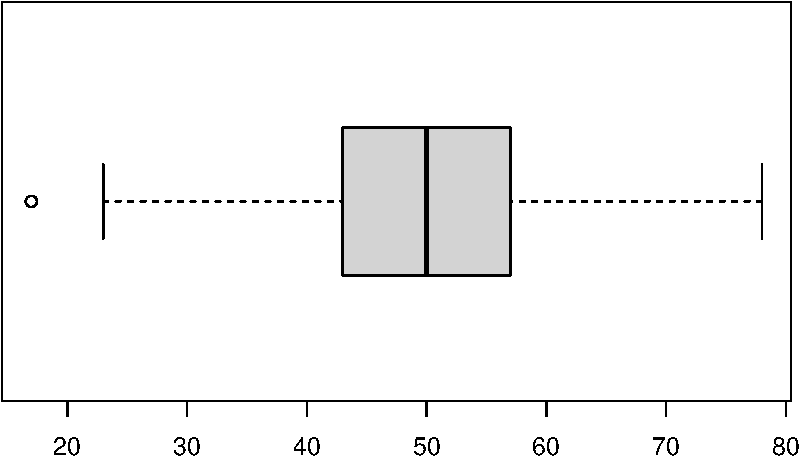
\includegraphics{A4_files/figure-latex/unnamed-chunk-12-1.pdf}

\begin{Shaded}
\begin{Highlighting}[]
\NormalTok{outliers }\OtherTok{=} \FunctionTok{boxplot.stats}\NormalTok{(df}\SpecialCharTok{$}\NormalTok{edad)}\SpecialCharTok{$}\NormalTok{out}
\FunctionTok{cat}\NormalTok{(}\StringTok{"Hay un total de"}\NormalTok{, }\FunctionTok{length}\NormalTok{(outliers), }\StringTok{"outliers en la variable edad"}\NormalTok{)}
\end{Highlighting}
\end{Shaded}

\begin{verbatim}
## Hay un total de 1 outliers en la variable edad
\end{verbatim}

\vspace{0.3cm}

Al único outlier encontrado, se le asigna NaN como valor y se muestra a
través de la función \emph{summary}.

\vspace{0.3cm}

\begin{Shaded}
\begin{Highlighting}[]
\NormalTok{df}\SpecialCharTok{$}\NormalTok{edad[}\FunctionTok{which}\NormalTok{(df}\SpecialCharTok{$}\NormalTok{edad }\SpecialCharTok{\%in\%}\NormalTok{ outliers)] }\OtherTok{=} \ConstantTok{NaN}
\FunctionTok{summary}\NormalTok{(df}\SpecialCharTok{$}\NormalTok{edad)}
\end{Highlighting}
\end{Shaded}

\begin{verbatim}
##    Min. 1st Qu.  Median    Mean 3rd Qu.    Max.    NA's 
##   23.00   43.00   50.00   49.89   57.00   78.00       1
\end{verbatim}

\vspace{0.3cm}

Al outlier se le imputa el de la media de la serie y se verifica
nuevamente cuántos outliers hay.

\vspace{0.3cm}

\begin{Shaded}
\begin{Highlighting}[]
\NormalTok{df}\SpecialCharTok{$}\NormalTok{edad[}\FunctionTok{is.na}\NormalTok{(df}\SpecialCharTok{$}\NormalTok{edad)] }\OtherTok{\textless{}{-}} \FunctionTok{mean}\NormalTok{(df}\SpecialCharTok{$}\NormalTok{edad, }\AttributeTok{na.rm =}\NormalTok{ T)}
\NormalTok{outliers }\OtherTok{=} \FunctionTok{boxplot.stats}\NormalTok{(df}\SpecialCharTok{$}\NormalTok{edad)}\SpecialCharTok{$}\NormalTok{out}
\FunctionTok{cat}\NormalTok{(}\StringTok{"Hay un total de"}\NormalTok{, }\FunctionTok{length}\NormalTok{(outliers), }\StringTok{"outliers en la variable edad"}\NormalTok{)}
\end{Highlighting}
\end{Shaded}

\begin{verbatim}
## Hay un total de 0 outliers en la variable edad
\end{verbatim}

\vspace{0.3cm}

Ahora bien, para el caso de la variable \emph{AE} se realiza otro
boxplot para verificar la existencia de outliers y contarlos.

\vspace{0.3cm}

\begin{Shaded}
\begin{Highlighting}[]
\NormalTok{outliers }\OtherTok{=} \FunctionTok{boxplot.stats}\NormalTok{(df}\SpecialCharTok{$}\NormalTok{AE)}\SpecialCharTok{$}\NormalTok{out}
\FunctionTok{cat}\NormalTok{(}\StringTok{"Hay un total de"}\NormalTok{, }\FunctionTok{length}\NormalTok{(outliers), }\StringTok{"outliers en la variable AE"}\NormalTok{)}
\end{Highlighting}
\end{Shaded}

\begin{verbatim}
## Hay un total de 4 outliers en la variable AE
\end{verbatim}

\begin{Shaded}
\begin{Highlighting}[]
\FunctionTok{boxplot}\NormalTok{(df}\SpecialCharTok{$}\NormalTok{AE, }\AttributeTok{horizontal =} \ConstantTok{TRUE}\NormalTok{)}
\end{Highlighting}
\end{Shaded}

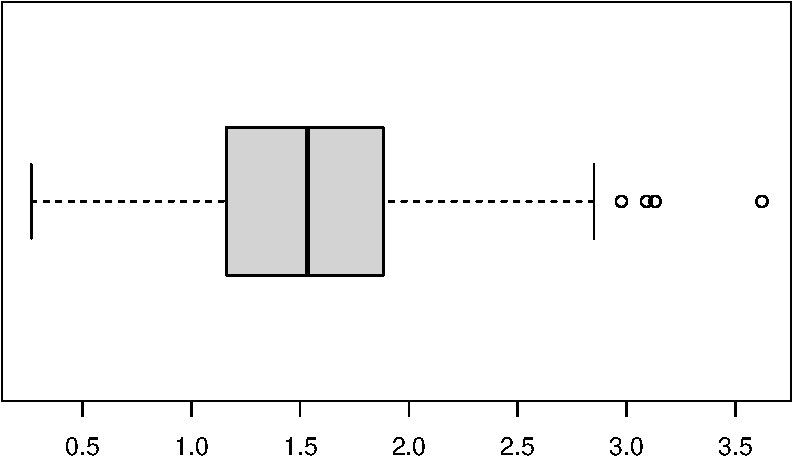
\includegraphics{A4_files/figure-latex/unnamed-chunk-15-1.pdf}

\vspace{0.3cm}

Se realiza el mismo procedimiento de imputación que para la variable
\emph{edad}, imputándole el valor de la media.

\vspace{0.3cm}

\begin{Shaded}
\begin{Highlighting}[]
\NormalTok{df}\SpecialCharTok{$}\NormalTok{AE[}\FunctionTok{is.na}\NormalTok{(df}\SpecialCharTok{$}\NormalTok{AE)] }\OtherTok{\textless{}{-}} \FunctionTok{mean}\NormalTok{(df}\SpecialCharTok{$}\NormalTok{AE, }\AttributeTok{na.rm =}\NormalTok{ T)}
\end{Highlighting}
\end{Shaded}

\vspace{0.3cm}

Estructura final del dataset procesado.

\vspace{0.3cm}

\begin{Shaded}
\begin{Highlighting}[]
\FunctionTok{summary}\NormalTok{(df)}
\end{Highlighting}
\end{Shaded}

\begin{verbatim}
##        AE         Tipo    genero       edad      
##  Min.   :0.2649   FI:41   F:144   Min.   :23.00  
##  1st Qu.:1.1618   FL:41   M:109   1st Qu.:43.00  
##  Median :1.5344   FM:39           Median :50.00  
##  Mean   :1.5493   FP:40           Mean   :49.89  
##  3rd Qu.:1.8824   NF:50           3rd Qu.:57.00  
##  Max.   :3.6226   NI:42           Max.   :78.00
\end{verbatim}

\newpage

\hypertarget{anuxe1lisis-de-la-muestra}{%
\section{2 Análisis de la muestra}\label{anuxe1lisis-de-la-muestra}}

\begin{center}\rule{0.5\linewidth}{0.5pt}\end{center}

\hypertarget{capacidad-pulmonar-y-guxe9nero}{%
\subsection{2.1 Capacidad pulmonar y
género}\label{capacidad-pulmonar-y-guxe9nero}}

\vspace{0.3cm}

Mostrar la capacidad pulmonar en relación al género. ¿Se observan
diferencias?

\vspace{0.3cm}

\begin{Shaded}
\begin{Highlighting}[]
\FunctionTok{ggplot}\NormalTok{(df, }\FunctionTok{aes}\NormalTok{(AE)) }\SpecialCharTok{+} \FunctionTok{geom\_histogram}\NormalTok{(}\FunctionTok{aes}\NormalTok{(}\AttributeTok{y =}\NormalTok{ ..density..), }\AttributeTok{bins =} \DecValTok{20}\NormalTok{,}
    \AttributeTok{color =} \StringTok{"black"}\NormalTok{, }\AttributeTok{fill =} \StringTok{"white"}\NormalTok{) }\SpecialCharTok{+} \FunctionTok{geom\_density}\NormalTok{(}\FunctionTok{aes}\NormalTok{(}\AttributeTok{fill =}\NormalTok{ genero),}
    \AttributeTok{alpha =} \FloatTok{0.2}\NormalTok{) }\SpecialCharTok{+} \FunctionTok{facet\_wrap}\NormalTok{(}\SpecialCharTok{\textasciitilde{}}\NormalTok{genero)}
\end{Highlighting}
\end{Shaded}

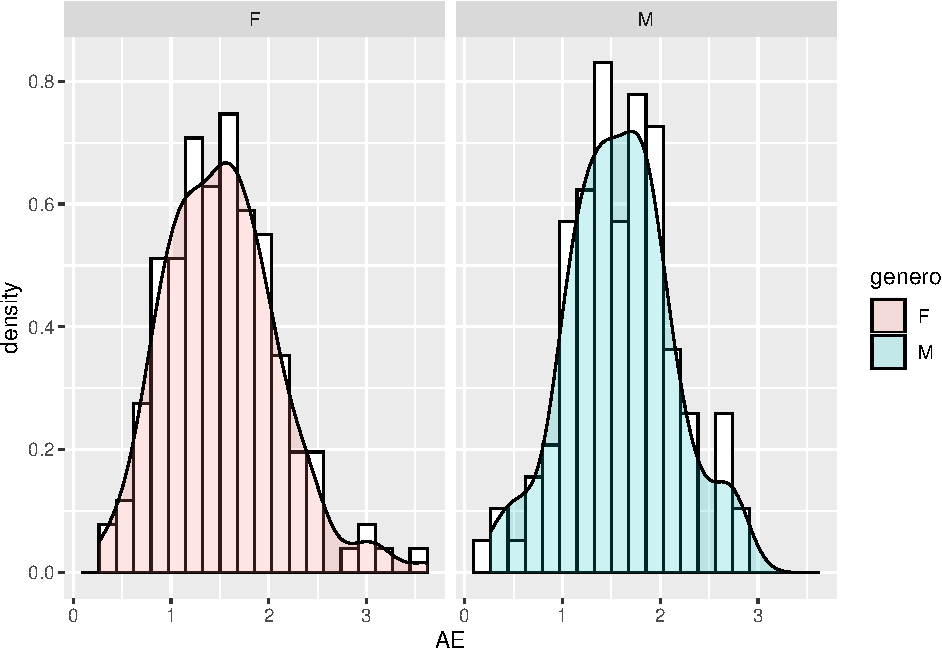
\includegraphics{A4_files/figure-latex/unnamed-chunk-18-1.pdf}

\vspace{0.3cm}

Las distribuciones parecen centradas en la media del intervalo
{[}0;3{]}, aunque sí existen más casos atípicos cuando el género es
\emph{F}.

\vspace{0.3cm}

\hypertarget{capacidad-pulmonar-y-edad}{%
\subsection{2.2 Capacidad pulmonar y
edad}\label{capacidad-pulmonar-y-edad}}

\vspace{0.3cm}

Mostrar la relación entre capacidad pulmonar y edad usando un gráfico de
dispersión. Interpretar.

\vspace{0.3cm}

\begin{Shaded}
\begin{Highlighting}[]
\FunctionTok{plot}\NormalTok{(df}\SpecialCharTok{$}\NormalTok{edad, df}\SpecialCharTok{$}\NormalTok{AE, }\AttributeTok{main =} \StringTok{"AE \textasciitilde{} edad"}\NormalTok{, }\AttributeTok{xlab =} \StringTok{"edad "}\NormalTok{, }\AttributeTok{ylab =} \StringTok{"AE "}\NormalTok{,}
    \AttributeTok{col =}\NormalTok{ df}\SpecialCharTok{$}\NormalTok{AE)}
\end{Highlighting}
\end{Shaded}

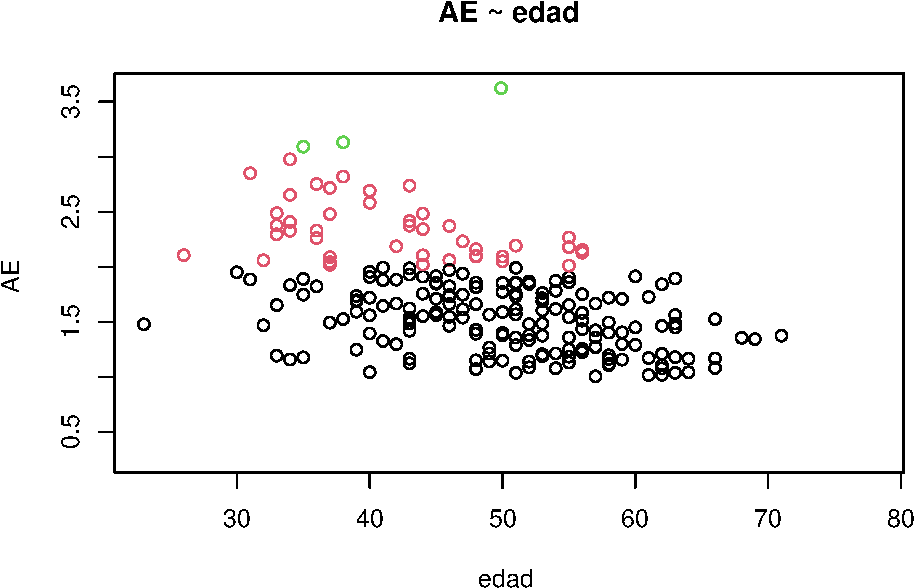
\includegraphics{A4_files/figure-latex/unnamed-chunk-19-1.pdf}

\hypertarget{tipos-de-fumadores-y-capacidad-pulmonar}{%
\subsection{2.3 Tipos de fumadores y capacidad
pulmonar}\label{tipos-de-fumadores-y-capacidad-pulmonar}}

\vspace{0.3cm}

Mostrar el número de personas en cada tipo de fumador y la media de AE
de cada tipo de fumador. Mostrad un gráfico que visualice esta media. Se
recomienda que el gráfico esté ordenado de menos a más AE.

\vspace{0.3cm}

\begin{Shaded}
\begin{Highlighting}[]
\FunctionTok{barplot}\NormalTok{(}\FunctionTok{table}\NormalTok{(df}\SpecialCharTok{$}\NormalTok{Tipo), }\AttributeTok{col =} \StringTok{"\#F7766C66"}\NormalTok{, }\AttributeTok{xlab =} \StringTok{"Tipo"}\NormalTok{, }\AttributeTok{ylab =} \StringTok{"Count"}\NormalTok{)}
\end{Highlighting}
\end{Shaded}

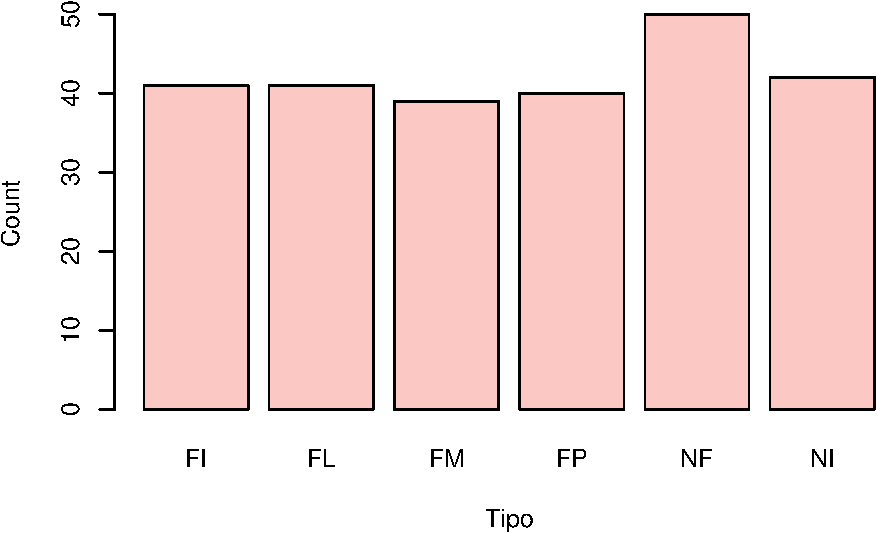
\includegraphics{A4_files/figure-latex/unnamed-chunk-20-1.pdf}

\newpage

Cálculo de la media de capacidad pulmonar \emph{AE} para cada tipo de
fumador.

\vspace{0.3cm}

\begin{Shaded}
\begin{Highlighting}[]
\NormalTok{resumen }\OtherTok{\textless{}{-}}\NormalTok{ df }\SpecialCharTok{\%\textgreater{}\%}
    \FunctionTok{group\_by}\NormalTok{(Tipo) }\SpecialCharTok{\%\textgreater{}\%}
    \FunctionTok{summarize}\NormalTok{(}\AttributeTok{means =} \FunctionTok{mean}\NormalTok{(AE), }\AttributeTok{counts =} \FunctionTok{length}\NormalTok{(AE))}
\FunctionTok{print}\NormalTok{(resumen)}
\end{Highlighting}
\end{Shaded}

\begin{verbatim}
## # A tibble: 6 x 3
##   Tipo  means counts
##   <fct> <dbl>  <int>
## 1 FI     1.22     41
## 2 FL     1.56     41
## 3 FM     1.16     39
## 4 FP     1.62     40
## 5 NF     1.99     50
## 6 NI     1.63     42
\end{verbatim}

\vspace{0.3cm}

Gráfico de las medias según el tipo de fumador.

\vspace{0.3cm}

\begin{Shaded}
\begin{Highlighting}[]
\FunctionTok{ggplot}\NormalTok{(resumen, }\FunctionTok{aes}\NormalTok{(}\AttributeTok{x =} \FunctionTok{reorder}\NormalTok{(Tipo, means), }\AttributeTok{y =}\NormalTok{ means)) }\SpecialCharTok{+} \FunctionTok{geom\_col}\NormalTok{(}\AttributeTok{fill =} \StringTok{"\#F7766C66"}\NormalTok{) }\SpecialCharTok{+}
    \FunctionTok{xlab}\NormalTok{(}\StringTok{"Tipo"}\NormalTok{) }\SpecialCharTok{+} \FunctionTok{ylab}\NormalTok{(}\StringTok{"Medias de AE"}\NormalTok{)}
\end{Highlighting}
\end{Shaded}

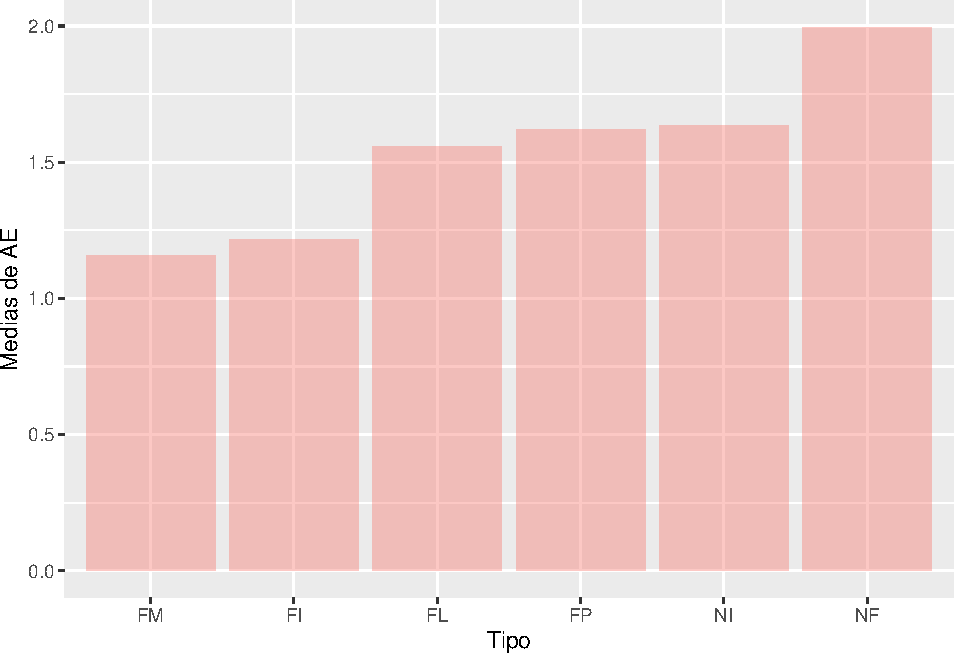
\includegraphics{A4_files/figure-latex/unnamed-chunk-22-1.pdf}

\newpage

Distribución de \emph{AE} según el tipo de fumador.

\vspace{0.3cm}

\begin{Shaded}
\begin{Highlighting}[]
\FunctionTok{ggplot}\NormalTok{(df, }\FunctionTok{aes}\NormalTok{(}\AttributeTok{x =}\NormalTok{ Tipo, }\AttributeTok{y =}\NormalTok{ AE)) }\SpecialCharTok{+} \FunctionTok{geom\_boxplot}\NormalTok{(}\AttributeTok{fill =} \StringTok{"\#F7766C66"}\NormalTok{)}
\end{Highlighting}
\end{Shaded}

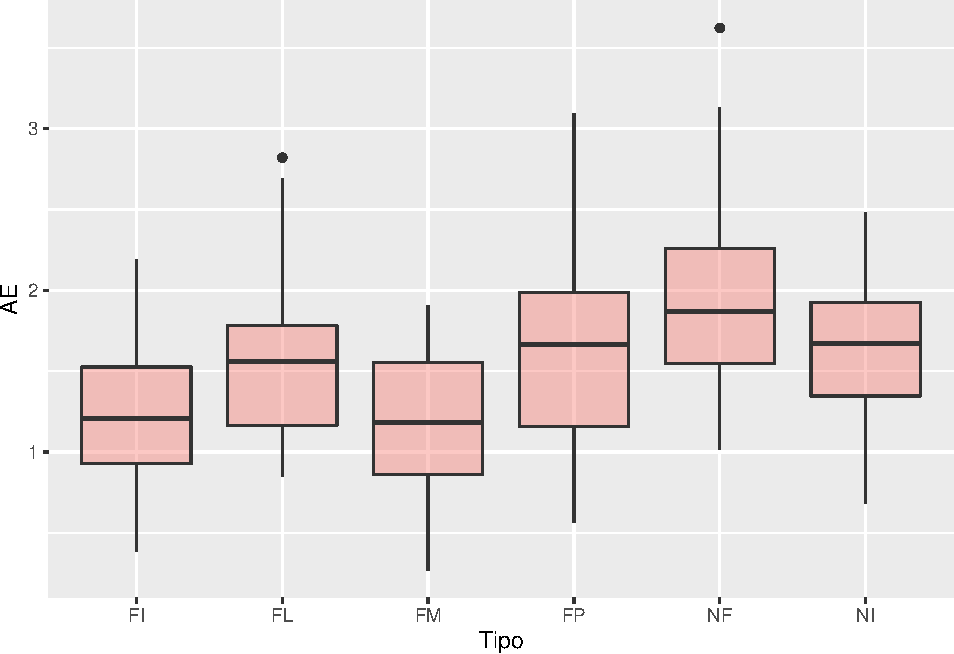
\includegraphics{A4_files/figure-latex/unnamed-chunk-23-1.pdf}

\vspace{0.3cm}

A partir del boxplot anterior, se puede ver que existen dos outliers en
la variable \emph{Tipo} cuando toma los valores FL y NF. Además, se
podría ver que la media de capacidad pulmonar para los No fumadores (NF)
es la más alta de todos los demás tipos y que podría haber una relación
entre los tipos FI y FM.

\newpage

\hypertarget{intervalo-de-confianza-de-la-capacidad-pulmonar}{%
\section{3 Intervalo de confianza de la capacidad
pulmonar}\label{intervalo-de-confianza-de-la-capacidad-pulmonar}}

\begin{center}\rule{0.5\linewidth}{0.5pt}\end{center}

\vspace{0.3cm}

Calcular el intervalo de confianza al 95\% de la capacidad pulmonar de
las mujeres y hombres por separado. Antes de aplicar el cálculo, revisar
si se cumplen las asunciones de aplicación del intervalo de confianza.
Interpretar los resultados. A partir de estos cálculos, ¿se observan
diferencias significativas en la capacidad pulmonar de mujeres y
hombres?

Nota: Realizar el cálculo manualmente sin usar las funciones t.test o
equivalentes. Podéis usar qnorm, qt, pnorm, pt, . . .

\vspace{0.3cm}

Se verifican las condiciones para la aplicación del intervalo de
confianza, donde se tiene un total de 253 registros en el dataset, con
109 casos masculinos y 144 casos Femeninos. Se tiene entonces más de 30
casos para cada tipo y una varianza descnocida, por lo que se verifica
así que puede construir a través de una distribución normal.

\vspace{0.3cm}

\begin{Shaded}
\begin{Highlighting}[]
\CommentTok{\# Función de cálculo del intervalo de confianza para}
\CommentTok{\# distribución normal}
\NormalTok{IC }\OtherTok{\textless{}{-}} \ControlFlowTok{function}\NormalTok{(x, NC) \{}
\NormalTok{    n }\OtherTok{\textless{}{-}} \FunctionTok{length}\NormalTok{(x)}
\NormalTok{    alpha }\OtherTok{\textless{}{-}} \DecValTok{1}\SpecialCharTok{/}\NormalTok{(NC}\SpecialCharTok{/}\DecValTok{100}\NormalTok{)}
\NormalTok{    SE }\OtherTok{\textless{}{-}} \FunctionTok{sd}\NormalTok{(x)}\SpecialCharTok{/}\FunctionTok{sqrt}\NormalTok{(n)}

\NormalTok{    z }\OtherTok{\textless{}{-}} \FunctionTok{qnorm}\NormalTok{(alpha}\SpecialCharTok{/}\DecValTok{2}\NormalTok{, }\AttributeTok{lower.tail =} \ConstantTok{TRUE}\NormalTok{)}
\NormalTok{    z\_SE }\OtherTok{\textless{}{-}}\NormalTok{ z }\SpecialCharTok{*}\NormalTok{ SE}
\NormalTok{    Low }\OtherTok{\textless{}{-}} \FunctionTok{mean}\NormalTok{(x) }\SpecialCharTok{{-}}\NormalTok{ z\_SE}
\NormalTok{    Up }\OtherTok{\textless{}{-}} \FunctionTok{mean}\NormalTok{(x) }\SpecialCharTok{+}\NormalTok{ z\_SE}

    \FunctionTok{return}\NormalTok{(}\FunctionTok{c}\NormalTok{(Low, Up))}
\NormalTok{\}}
\end{Highlighting}
\end{Shaded}

\vspace{0.3cm}

\begin{Shaded}
\begin{Highlighting}[]
\NormalTok{int\_conf\_f }\OtherTok{\textless{}{-}} \FunctionTok{IC}\NormalTok{(df}\SpecialCharTok{$}\NormalTok{AE[df}\SpecialCharTok{$}\NormalTok{genero }\SpecialCharTok{==} \StringTok{"F"}\NormalTok{], }\DecValTok{95}\NormalTok{)}
\NormalTok{int\_conf\_m }\OtherTok{\textless{}{-}} \FunctionTok{IC}\NormalTok{(df}\SpecialCharTok{$}\NormalTok{AE[df}\SpecialCharTok{$}\NormalTok{genero }\SpecialCharTok{==} \StringTok{"M"}\NormalTok{], }\DecValTok{95}\NormalTok{)}
\end{Highlighting}
\end{Shaded}

\vspace{0.3cm}

El intervalo de confianza al 95\% para el género M es {[}1.5803834,
1.5871413{]} mientras que para el género F es {[}1.5201125,
1.5264477{]}.

\vspace{0.3cm}

Ambos intervalos son relativamente similares puesto que varían recién en
la segunda cifra decimal, ambos rondan el 1.55 como valor central.

\newpage

\hypertarget{diferencias-en-capacidad-pulmonar-entre-mujeres-y-hombres}{%
\section{4 Diferencias en capacidad pulmonar entre mujeres y
hombres}\label{diferencias-en-capacidad-pulmonar-entre-mujeres-y-hombres}}

\begin{center}\rule{0.5\linewidth}{0.5pt}\end{center}

\vspace{0.3cm}

Aplicar un contraste de hipótesis para evaluar si existen diferencias
significativas entre la capacidad pulmonar de mujeres y hombres. Seguid
los pasos que se indican a continuación.

Nota: Realizar el cálculo manualmente sin usar las funciones t.test o
equivalentes. Podéis usar qnorm, qt, pnorm, pt, . . .

\vspace{0.3cm}

\hypertarget{hipuxf3tesis}{%
\subsection{4.1 Hipótesis}\label{hipuxf3tesis}}

Escribir la hipótesis nula y alternativa.

\vspace{0.3cm}

\[H_0:  \mu_{AE\_M} = \mu_{AE\_F}\]
\[H_1: \mu_{AE\_M} \neq \mu_{AE\_F}\]

\vspace{0.3cm}

\hypertarget{contraste}{%
\subsection{4.2 Contraste}\label{contraste}}

Explicad qué tipo de contraste aplicaréis y por qué. Si es necesario,
validad las asunciones del test.

\vspace{0.3cm}

Se utiliza para este apartado un contraste de media de dos
distribuciones, porque son dos separadas, independientes una de la otra
aunque ambas pertenecen a la misma muestra.

\vspace{0.3cm}

\begin{Shaded}
\begin{Highlighting}[]
\NormalTok{contraste\_medias }\OtherTok{\textless{}{-}} \ControlFlowTok{function}\NormalTok{(s1, s2, alt, CL) \{}

    \CommentTok{\# Cálculo de Medias}
\NormalTok{    mean1 }\OtherTok{\textless{}{-}} \FunctionTok{mean}\NormalTok{(s1)}
\NormalTok{    mean2 }\OtherTok{\textless{}{-}} \FunctionTok{mean}\NormalTok{(s2)}

    \CommentTok{\# Cálculo del tamaño de la muestra}
\NormalTok{    n1 }\OtherTok{\textless{}{-}} \FunctionTok{length}\NormalTok{(s1)}
\NormalTok{    n2 }\OtherTok{\textless{}{-}} \FunctionTok{length}\NormalTok{(s2)}

    \CommentTok{\# Cálculo de la desviación estándar}
\NormalTok{    sd1 }\OtherTok{\textless{}{-}} \FunctionTok{sd}\NormalTok{(s1)}
\NormalTok{    sd2 }\OtherTok{\textless{}{-}} \FunctionTok{sd}\NormalTok{(s2)}

    \CommentTok{\# Cálculo del nivel de significancia}
\NormalTok{    alpha }\OtherTok{\textless{}{-}}\NormalTok{ (}\DecValTok{1} \SpecialCharTok{{-}}\NormalTok{ CL}\SpecialCharTok{/}\DecValTok{100}\NormalTok{)}

    \CommentTok{\# Cálculo de los grados de libertad (Apartado 5.2.2 de}
    \CommentTok{\# la teoría)}
\NormalTok{    denominador }\OtherTok{\textless{}{-}}\NormalTok{ ((sd1}\SpecialCharTok{\^{}}\DecValTok{2}\SpecialCharTok{/}\NormalTok{n1)}\SpecialCharTok{\^{}}\DecValTok{2}\SpecialCharTok{/}\NormalTok{(n1 }\SpecialCharTok{{-}} \DecValTok{1}\NormalTok{) }\SpecialCharTok{+}\NormalTok{ (sd2}\SpecialCharTok{\^{}}\DecValTok{2}\SpecialCharTok{/}\NormalTok{n2)}\SpecialCharTok{\^{}}\DecValTok{2}\SpecialCharTok{/}\NormalTok{(n2 }\SpecialCharTok{{-}}
        \DecValTok{1}\NormalTok{))}
\NormalTok{    df }\OtherTok{\textless{}{-}}\NormalTok{ ((sd1}\SpecialCharTok{\^{}}\DecValTok{2}\SpecialCharTok{/}\NormalTok{n1 }\SpecialCharTok{+}\NormalTok{ sd2}\SpecialCharTok{\^{}}\DecValTok{2}\SpecialCharTok{/}\NormalTok{n2)}\SpecialCharTok{\^{}}\DecValTok{2}\NormalTok{)}\SpecialCharTok{/}\NormalTok{denominador}

    \CommentTok{\# Cálculo del valor t (z según la distribución normal}
    \CommentTok{\# estandarizada)}
\NormalTok{    sb }\OtherTok{\textless{}{-}} \FunctionTok{sqrt}\NormalTok{(sd1}\SpecialCharTok{\^{}}\DecValTok{2}\SpecialCharTok{/}\NormalTok{n1 }\SpecialCharTok{+}\NormalTok{ sd2}\SpecialCharTok{\^{}}\DecValTok{2}\SpecialCharTok{/}\NormalTok{n2)}
\NormalTok{    t }\OtherTok{\textless{}{-}}\NormalTok{ (mean1 }\SpecialCharTok{{-}}\NormalTok{ mean2)}\SpecialCharTok{/}\NormalTok{sb}

    \CommentTok{\# Evaluación de la condición =}
    \ControlFlowTok{if}\NormalTok{ (alt }\SpecialCharTok{==} \StringTok{"bilateral"}\NormalTok{) \{}
\NormalTok{        t\_critical }\OtherTok{\textless{}{-}} \FunctionTok{qt}\NormalTok{(alpha}\SpecialCharTok{/}\DecValTok{2}\NormalTok{, df, }\AttributeTok{lower.tail =} \ConstantTok{FALSE}\NormalTok{)}
\NormalTok{        p\_value }\OtherTok{\textless{}{-}} \FunctionTok{pt}\NormalTok{(}\FunctionTok{abs}\NormalTok{(t), df, }\AttributeTok{lower.tail =} \ConstantTok{FALSE}\NormalTok{) }\SpecialCharTok{*} \DecValTok{2}

        \CommentTok{\# Evaluación de la condición \textless{}}
\NormalTok{    \} }\ControlFlowTok{else} \ControlFlowTok{if}\NormalTok{ (alt }\SpecialCharTok{==} \StringTok{"\textless{}"}\NormalTok{) \{}
\NormalTok{        t\_critical }\OtherTok{\textless{}{-}} \FunctionTok{qt}\NormalTok{(alpha, df, }\AttributeTok{lower.tail =} \ConstantTok{TRUE}\NormalTok{)}
\NormalTok{        p\_value }\OtherTok{\textless{}{-}} \FunctionTok{pt}\NormalTok{(t, df, }\AttributeTok{lower.tail =} \ConstantTok{TRUE}\NormalTok{)}

        \CommentTok{\# Evaluación de la condición \textgreater{} (alt == \textquotesingle{}\textgreater{}\textquotesingle{})}
\NormalTok{    \} }\ControlFlowTok{else}\NormalTok{ \{}
\NormalTok{        t\_critical }\OtherTok{\textless{}{-}} \FunctionTok{qt}\NormalTok{(alpha, df, }\AttributeTok{lower.tail =} \ConstantTok{FALSE}\NormalTok{)}
\NormalTok{        p\_value }\OtherTok{\textless{}{-}} \FunctionTok{pt}\NormalTok{(t, df, }\AttributeTok{lower.tail =} \ConstantTok{FALSE}\NormalTok{)}
\NormalTok{    \}}

    \CommentTok{\# Definición del vector resultado}
\NormalTok{    vector\_data }\OtherTok{\textless{}{-}} \FunctionTok{c}\NormalTok{(mean1, mean2, t, t\_critical, p\_value, alpha,}
\NormalTok{        df)}
    \FunctionTok{names}\NormalTok{(vector\_data) }\OtherTok{\textless{}{-}} \FunctionTok{c}\NormalTok{(}\StringTok{"mean1"}\NormalTok{, }\StringTok{"mean2"}\NormalTok{, }\StringTok{"t"}\NormalTok{, }\StringTok{"t\_critical"}\NormalTok{,}
        \StringTok{"p\_value"}\NormalTok{, }\StringTok{"alpha"}\NormalTok{, }\StringTok{"df"}\NormalTok{)}
    \FunctionTok{return}\NormalTok{(vector\_data)}
\NormalTok{\}}
\end{Highlighting}
\end{Shaded}

\vspace{0.3cm}

\hypertarget{cuxe1lculos}{%
\subsection{4.3 Cálculos}\label{cuxe1lculos}}

Aplicad los cálculos del contraste. Mostrar el valor observado, el valor
de contraste y el valor p.

\vspace{0.3cm}

\begin{Shaded}
\begin{Highlighting}[]
\NormalTok{x }\OtherTok{\textless{}{-}}\NormalTok{ df}\SpecialCharTok{$}\NormalTok{AE[df}\SpecialCharTok{$}\NormalTok{genero }\SpecialCharTok{==} \StringTok{"F"}\NormalTok{]}
\NormalTok{y }\OtherTok{\textless{}{-}}\NormalTok{ df}\SpecialCharTok{$}\NormalTok{AE[df}\SpecialCharTok{$}\NormalTok{genero }\SpecialCharTok{==} \StringTok{"M"}\NormalTok{]}
\NormalTok{datos }\OtherTok{\textless{}{-}} \FunctionTok{contraste\_medias}\NormalTok{(x, y, }\StringTok{"bilateral"}\NormalTok{, }\DecValTok{95}\NormalTok{)}
\FunctionTok{vertical}\NormalTok{(datos)}
\end{Highlighting}
\end{Shaded}

\begin{verbatim}
##                   [,1]
## mean1        1.5232801
## mean2        1.5837624
## t           -0.8620365
## t_critical   1.9698650
## p_value      0.3895251
## alpha        0.0500000
## df         240.7863233
\end{verbatim}

\vspace{0.3cm}

\hypertarget{cuxe1lculos-1}{%
\subsection{4.3 Cálculos}\label{cuxe1lculos-1}}

Interpretad los resultados y comparad las conclusiones con los
intervalos de confianza calculados anteriormente.

\vspace{0.3cm}

Como el \emph{p\_value} es mayor que el nivel de significancia, se debe
aceptar la hipótesis nula porque no hay evidencia suficiente para poder
descartarla. Por lo tanto, lo único que se puede decir es que la
capacidad pulmonar de ambos grupos se muestra igual.

\newpage

\hypertarget{diferencias-en-la-capacidad-pulmonar-entre-fumadores-y-no-fumadores}{%
\section{5 Diferencias en la capacidad pulmonar entre Fumadores y No
Fumadores}\label{diferencias-en-la-capacidad-pulmonar-entre-fumadores-y-no-fumadores}}

\begin{center}\rule{0.5\linewidth}{0.5pt}\end{center}

\vspace{0.3cm}

¿Podemos afirmar que la capacidad pulmonar de los fumadores es inferior
a la de no fumadores? Incluid dentro de la categoría de no fumadores los
fumadores pasivos. Seguid los pasos que se indican a continuación.

Nota: Realizar el cálculo manualmente sin usar las funciones t.test o
equivalentes. Podéis usar qnorm, qt, pnorm, pt, . . .

\vspace{0.3cm}

\hypertarget{hipuxf3tesis-1}{%
\subsection{5.1 Hipótesis}\label{hipuxf3tesis-1}}

Escribir la hipótesis nula y alternativa.

\vspace{0.3cm}

\[H_0:  \mu_{AE\_FUM} \geq \mu_{AE\_NOFUM}\]
\[H_1: \mu_{AE\_FUM} < \mu_{AE\_NOFUM}\]

\vspace{0.3cm}

\hypertarget{contraste-1}{%
\subsection{5.2 Contraste}\label{contraste-1}}

Explicad qué tipo de contraste aplicaréis y por qué. Si es necesario,
validad las asunciones del test.

\vspace{0.3cm}

Se aplica un contraste de hipótesis de dos muestras independientes, ya
que hay suficientes casos en cada distribución para poder afirmar que
siguen una distribución normal. Además, se tienen varianzas
poblacionales desconocidas diferentes.

\vspace{0.3cm}

\hypertarget{preparaciuxf3n-de-los-datos}{%
\subsection{5.3 Preparación de los
datos}\label{preparaciuxf3n-de-los-datos}}

Preparad las muestras. Una de ellas contiene los valores de AE de los
fumadores y la otra, los valores de AE de los no fumadores y fumadores
pasivos.

\vspace{0.3cm}

\begin{Shaded}
\begin{Highlighting}[]
\NormalTok{indeces }\OtherTok{\textless{}{-}}\NormalTok{ df}\SpecialCharTok{$}\NormalTok{Tipo }\SpecialCharTok{==} \StringTok{"NF"} \SpecialCharTok{|}\NormalTok{ df}\SpecialCharTok{$}\NormalTok{Tipo }\SpecialCharTok{==} \StringTok{"FP"}
\NormalTok{no\_fumadores }\OtherTok{\textless{}{-}}\NormalTok{ df}\SpecialCharTok{$}\NormalTok{AE[indeces]}
\NormalTok{fumadores }\OtherTok{\textless{}{-}}\NormalTok{ df}\SpecialCharTok{$}\NormalTok{AE[}\SpecialCharTok{!}\NormalTok{indeces]}
\FunctionTok{cat}\NormalTok{(}\StringTok{"No Fumadores: "}\NormalTok{, }\FunctionTok{length}\NormalTok{(no\_fumadores))}
\end{Highlighting}
\end{Shaded}

\begin{verbatim}
## No Fumadores:  90
\end{verbatim}

\begin{Shaded}
\begin{Highlighting}[]
\FunctionTok{cat}\NormalTok{(}\StringTok{"Fumadores: "}\NormalTok{, }\FunctionTok{length}\NormalTok{(fumadores))}
\end{Highlighting}
\end{Shaded}

\begin{verbatim}
## Fumadores:  163
\end{verbatim}

\newpage

\hypertarget{cuxe1lculos-2}{%
\subsection{5.4 Cálculos}\label{cuxe1lculos-2}}

Preparad las muestras. Una de ellas contiene los valores de AE de los
fumadores y la otra, los valores de AE de los no fumadores y fumadores
pasivos.

\vspace{0.3cm}

\begin{Shaded}
\begin{Highlighting}[]
\NormalTok{datos }\OtherTok{\textless{}{-}} \FunctionTok{contraste\_medias}\NormalTok{(fumadores, no\_fumadores, }\StringTok{"\textless{}"}\NormalTok{, }\DecValTok{95}\NormalTok{)}
\FunctionTok{vertical}\NormalTok{(datos)}
\end{Highlighting}
\end{Shaded}

\begin{verbatim}
##                     [,1]
## mean1       1.395786e+00
## mean2       1.827437e+00
## t          -6.128091e+00
## t_critical -1.654029e+00
## p_value     3.095169e-09
## alpha       5.000000e-02
## df          1.669948e+02
\end{verbatim}

\vspace{0.3cm}

\hypertarget{interpretaciuxf3n}{%
\subsection{5.5 Interpretación}\label{interpretaciuxf3n}}

Interpretar el resultado del contraste

\vspace{0.3cm}

Ya que el \emph{p\_value} tiene un valor menor al nivel de
significancia, se puede rechazar la hipótesis nula y aceptar la
hipótesis alternativa. Por lo tanto, se tiene evidencia estadística
suficiente para inferir que la capacidad pulmonar de los fumadores es
menor que la de los no fumadores.

\newpage

\hypertarget{anuxe1lisis-de-regresiuxf3n-lineal}{%
\section{6 Análisis de regresión
lineal}\label{anuxe1lisis-de-regresiuxf3n-lineal}}

\begin{center}\rule{0.5\linewidth}{0.5pt}\end{center}

\vspace{0.3cm}

Realizamos un análisis de regresión lineal para investigar la relación
entre la variable capacidad pulmonar (AE) y el resto de variables (tipo,
edad y género). Construid e interpretad el modelo, siguiendo los pasos
que se especifican a continuación.

\vspace{0.3cm}

\hypertarget{cuxe1lculo}{%
\subsection{6.1 Cálculo}\label{cuxe1lculo}}

Calculad el modelo de regresión lineal. Podéis usar la función lm.

\vspace{0.3cm}

\begin{Shaded}
\begin{Highlighting}[]
\NormalTok{model }\OtherTok{\textless{}{-}} \FunctionTok{lm}\NormalTok{(}\AttributeTok{formula =}\NormalTok{ AE }\SpecialCharTok{\textasciitilde{}}\NormalTok{ Tipo }\SpecialCharTok{+}\NormalTok{ edad }\SpecialCharTok{+}\NormalTok{ genero, df)}
\FunctionTok{summary}\NormalTok{(model)}
\end{Highlighting}
\end{Shaded}

\begin{verbatim}
## 
## Call:
## lm(formula = AE ~ Tipo + edad + genero, data = df)
## 
## Residuals:
##      Min       1Q   Median       3Q      Max 
## -1.05722 -0.24940 -0.00566  0.22740  1.62120 
## 
## Coefficients:
##              Estimate Std. Error t value Pr(>|t|)    
## (Intercept)  2.704758   0.135750  19.924  < 2e-16 ***
## TipoFL       0.337958   0.083609   4.042 7.10e-05 ***
## TipoFM       0.043769   0.084954   0.515    0.607    
## TipoFP       0.395316   0.084249   4.692 4.50e-06 ***
## TipoNF       0.801520   0.079657  10.062  < 2e-16 ***
## TipoNI       0.423578   0.082998   5.103 6.69e-07 ***
## edad        -0.030162   0.002407 -12.533  < 2e-16 ***
## generoM     -0.007653   0.048702  -0.157    0.875    
## ---
## Signif. codes:  0 '***' 0.001 '**' 0.01 '*' 0.05 '.' 0.1 ' ' 1
## 
## Residual standard error: 0.3779 on 245 degrees of freedom
## Multiple R-squared:  0.5541, Adjusted R-squared:  0.5414 
## F-statistic: 43.49 on 7 and 245 DF,  p-value: < 2.2e-16
\end{verbatim}

\vspace{0.3cm}

\hypertarget{interpretaciuxf3n-1}{%
\subsection{6.2 Interpretación}\label{interpretaciuxf3n-1}}

Interpretad el modelo y la contribución de cada variable explicativa
sobre la variable AE.

\vspace{0.3cm}

\begin{itemize}
\tightlist
\item
  el \emph{p\_value} es de 2.26e-16, es decir, que podemos considerar
  que se ha obtenido una muy buena regresión ya que está muy por debajo
  del nivel de significación.
\item
  la \emph{recta de regresión} que se desprende de la información del
  modelo es \emph{y = 2.704758 + 0.337958 * TipoFL + 0.043769 * TipoFM +
  0.395316 * TipoFP + 0.801520 * TipoNF + 0.423578 * TipoNI - 0.030162 *
  edad - 0.007653 * generoM}
\item
  para un nivel de significancia de 0.05, las variables TipoFM y generoM
  tienen un valor \emph{Pr(\textgreater\textbar t\textbar)} mayor que el
  nivel de significancia, por lo que no son relevantes para el modelo.
\end{itemize}

\newpage

\hypertarget{bondad-del-ajuste}{%
\subsection{6.3 Bondad del ajuste}\label{bondad-del-ajuste}}

Evaluad la calidad del modelo.

\vspace{0.3cm}

El \emph{R-quared} tiene un valor de 0.5541, por lo que no se podría
decir que es un modelo ajustado ya que está alejado del 1, pero tampoco
es poco ajustado porque está alejado del 0.

\vspace{0.3cm}

\hypertarget{predicciuxf3n}{%
\subsection{6.4 Predicción}\label{predicciuxf3n}}

Realizad una predicción de la capacidad pulmonar para cada tipo de
fumador desde los 30 años de edad hasta los 80 años de edad (podéis
asumir género hombre). Mostrad una tabla con los resultados. Mostrad
también visualmente la simulación.

\vspace{0.3cm}

\begin{Shaded}
\begin{Highlighting}[]
\FunctionTok{names}\NormalTok{(tipos) }\OtherTok{\textless{}{-}}\NormalTok{ tipos}
\NormalTok{edades }\OtherTok{\textless{}{-}} \DecValTok{30}\SpecialCharTok{:}\DecValTok{80}
\FunctionTok{names}\NormalTok{(edades) }\OtherTok{\textless{}{-}}\NormalTok{ edades}
\NormalTok{predictions }\OtherTok{\textless{}{-}} \FunctionTok{data.frame}\NormalTok{(}\FunctionTok{outer}\NormalTok{(edades, tipos, }\ControlFlowTok{function}\NormalTok{(edad,}
\NormalTok{    tipo) \{}
    \FunctionTok{return}\NormalTok{(}\FunctionTok{predict}\NormalTok{(model, }\FunctionTok{data.frame}\NormalTok{(}\AttributeTok{Tipo =}\NormalTok{ tipo, }\AttributeTok{edad =}\NormalTok{ edad,}
        \AttributeTok{genero =} \StringTok{"M"}\NormalTok{)))}
\NormalTok{\}))}
\NormalTok{predictions[}\StringTok{"edades"}\NormalTok{] }\OtherTok{\textless{}{-}}\NormalTok{ edades}
\NormalTok{predictions}
\end{Highlighting}
\end{Shaded}

\begin{verbatim}
##          NF        FP        NI        FL        FM        FI edades
## 30 2.593771 2.1875670 2.2158288 2.1302092 1.8360199 1.7922509     30
## 31 2.563609 2.1574052 2.1856670 2.1000474 1.8058581 1.7620891     31
## 32 2.533447 2.1272434 2.1555052 2.0698855 1.7756963 1.7319272     32
## 33 2.503285 2.0970816 2.1253433 2.0397237 1.7455345 1.7017654     33
## 34 2.473124 2.0669197 2.0951815 2.0095619 1.7153726 1.6716036     34
## 35 2.442962 2.0367579 2.0650197 1.9794001 1.6852108 1.6414418     35
## 36 2.412800 2.0065961 2.0348579 1.9492382 1.6550490 1.6112799     36
## 37 2.382638 1.9764343 2.0046960 1.9190764 1.6248872 1.5811181     37
## 38 2.352476 1.9462724 1.9745342 1.8889146 1.5947253 1.5509563     38
## 39 2.322314 1.9161106 1.9443724 1.8587528 1.5645635 1.5207945     39
## 40 2.292153 1.8859488 1.9142106 1.8285909 1.5344017 1.4906326     40
## 41 2.261991 1.8557870 1.8840487 1.7984291 1.5042399 1.4604708     41
## 42 2.231829 1.8256251 1.8538869 1.7682673 1.4740780 1.4303090     42
## 43 2.201667 1.7954633 1.8237251 1.7381055 1.4439162 1.4001472     43
## 44 2.171505 1.7653015 1.7935633 1.7079436 1.4137544 1.3699853     44
## 45 2.141344 1.7351397 1.7634014 1.6777818 1.3835926 1.3398235     45
## 46 2.111182 1.7049778 1.7332396 1.6476200 1.3534307 1.3096617     46
## 47 2.081020 1.6748160 1.7030778 1.6174582 1.3232689 1.2794999     47
## 48 2.050858 1.6446542 1.6729160 1.5872963 1.2931071 1.2493380     48
## 49 2.020696 1.6144924 1.6427541 1.5571345 1.2629453 1.2191762     49
## 50 1.990534 1.5843305 1.6125923 1.5269727 1.2327834 1.1890144     50
## 51 1.960373 1.5541687 1.5824305 1.4968109 1.2026216 1.1588526     51
## 52 1.930211 1.5240069 1.5522687 1.4666490 1.1724598 1.1286907     52
## 53 1.900049 1.4938451 1.5221068 1.4364872 1.1422980 1.0985289     53
## 54 1.869887 1.4636832 1.4919450 1.4063254 1.1121361 1.0683671     54
## 55 1.839725 1.4335214 1.4617832 1.3761636 1.0819743 1.0382053     55
## 56 1.809563 1.4033596 1.4316214 1.3460017 1.0518125 1.0080434     56
## 57 1.779402 1.3731978 1.4014595 1.3158399 1.0216507 0.9778816     57
## 58 1.749240 1.3430359 1.3712977 1.2856781 0.9914888 0.9477198     58
## 59 1.719078 1.3128741 1.3411359 1.2555163 0.9613270 0.9175580     59
## 60 1.688916 1.2827123 1.3109741 1.2253544 0.9311652 0.8873961     60
## 61 1.658754 1.2525505 1.2808122 1.1951926 0.9010034 0.8572343     61
## 62 1.628593 1.2223886 1.2506504 1.1650308 0.8708415 0.8270725     62
## 63 1.598431 1.1922268 1.2204886 1.1348690 0.8406797 0.7969107     63
## 64 1.568269 1.1620650 1.1903268 1.1047071 0.8105179 0.7667488     64
## 65 1.538107 1.1319032 1.1601649 1.0745453 0.7803561 0.7365870     65
## 66 1.507945 1.1017413 1.1300031 1.0443835 0.7501942 0.7064252     66
## 67 1.477783 1.0715795 1.0998413 1.0142217 0.7200324 0.6762634     67
## 68 1.447622 1.0414177 1.0696795 0.9840598 0.6898706 0.6461015     68
## 69 1.417460 1.0112559 1.0395176 0.9538980 0.6597088 0.6159397     69
## 70 1.387298 0.9810940 1.0093558 0.9237362 0.6295469 0.5857779     70
## 71 1.357136 0.9509322 0.9791940 0.8935744 0.5993851 0.5556161     71
## 72 1.326974 0.9207704 0.9490322 0.8634125 0.5692233 0.5254542     72
## 73 1.296812 0.8906086 0.9188703 0.8332507 0.5390615 0.4952924     73
## 74 1.266651 0.8604467 0.8887085 0.8030889 0.5088996 0.4651306     74
## 75 1.236489 0.8302849 0.8585467 0.7729271 0.4787378 0.4349688     75
## 76 1.206327 0.8001231 0.8283849 0.7427652 0.4485760 0.4048069     76
## 77 1.176165 0.7699613 0.7982230 0.7126034 0.4184142 0.3746451     77
## 78 1.146003 0.7397994 0.7680612 0.6824416 0.3882523 0.3444833     78
## 79 1.115841 0.7096376 0.7378994 0.6522798 0.3580905 0.3143215     79
## 80 1.085680 0.6794758 0.7077376 0.6221179 0.3279287 0.2841596     80
\end{verbatim}

\vspace{0.3cm}

\begin{Shaded}
\begin{Highlighting}[]
\NormalTok{predictions.melt }\OtherTok{\textless{}{-}} \FunctionTok{melt}\NormalTok{(predictions, }\AttributeTok{id.vars =} \StringTok{"edades"}\NormalTok{)}
\FunctionTok{ggplot}\NormalTok{(predictions.melt, }\FunctionTok{aes}\NormalTok{(edades, value, }\AttributeTok{colour =}\NormalTok{ variable)) }\SpecialCharTok{+}
    \FunctionTok{geom\_point}\NormalTok{() }\SpecialCharTok{+} \FunctionTok{ylab}\NormalTok{(}\StringTok{"AE"}\NormalTok{) }\SpecialCharTok{+} \FunctionTok{labs}\NormalTok{(}\AttributeTok{color =} \StringTok{"Tipos"}\NormalTok{)}
\end{Highlighting}
\end{Shaded}

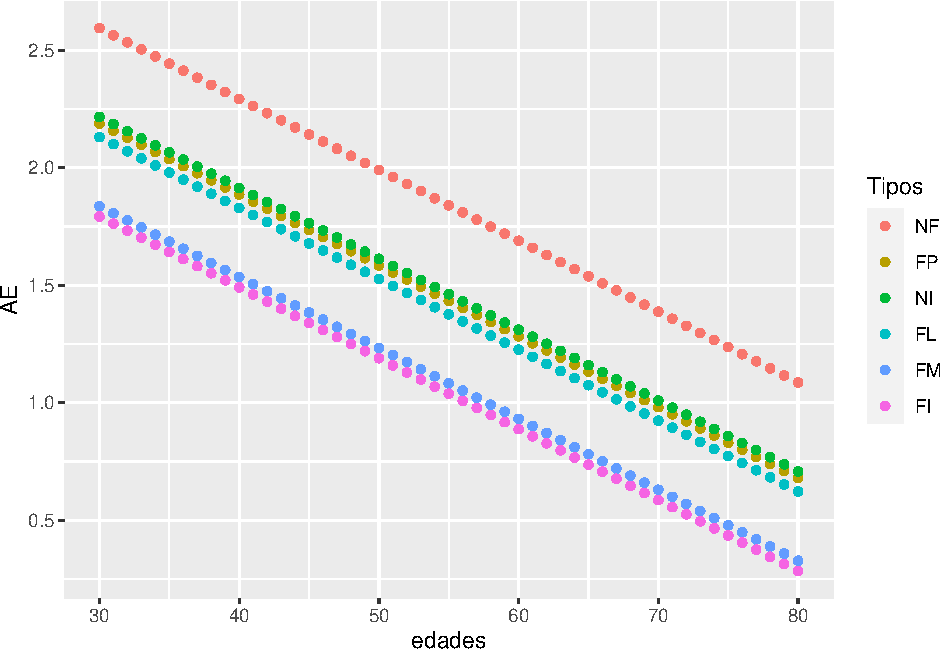
\includegraphics{A4_files/figure-latex/unnamed-chunk-32-1.pdf}

\newpage

\hypertarget{anova-unifactorial}{%
\section{7 ANOVA unifactorial}\label{anova-unifactorial}}

\begin{center}\rule{0.5\linewidth}{0.5pt}\end{center}

\vspace{0.3cm}

A continuación se realizará un análisis de varianza, donde se desea
comparar la capacidad pulmonar entre los seis tipos de fumadores/no
fumadores clasificados previamente. El análisis de varianza consiste en
evaluar si la variabilidad de una variable dependiente puede explicarse
a partir de una o varias variables independientes, denominadas factores.
En el caso que nos ocupa, nos interesa evaluar si la variabilidad de la
variable AE puede explicarse por el factor tipo de fumador. Hay dos
preguntas básicas a responder:

\begin{itemize}
\tightlist
\item
  ¿Existen diferencias entre la capacidad pulmonar (AE) entre los
  distintos tipos de fumadores/no fumadores?
\item
  Si existen diferencias, ¿entre qué grupos están estas diferencias?
\end{itemize}

\vspace{0.3cm}

\hypertarget{normalidad}{%
\subsection{7.1 Normalidad}\label{normalidad}}

Evaluar si el conjunto de datos cumple las condiciones de aplicación de
ANOVA. Seguid los pasos que se indican a continuación. Mostrad
visualmente si existe normalidad en los datos y también aplicar un test
de normalidad.

Nota: podéis usar el gráfico normal Q-Q y el test Shapiro-Wilk para
evaluar la normalidad de los residuos.

\vspace{0.3cm}

\begin{Shaded}
\begin{Highlighting}[]
\NormalTok{linear\_model }\OtherTok{\textless{}{-}} \FunctionTok{lm}\NormalTok{(AE }\SpecialCharTok{\textasciitilde{}}\NormalTok{ Tipo, df)}
\NormalTok{linear\_residuals }\OtherTok{\textless{}{-}} \FunctionTok{residuals}\NormalTok{(linear\_model)}
\FunctionTok{qqnorm}\NormalTok{(linear\_residuals)}
\FunctionTok{qqline}\NormalTok{(linear\_residuals)}
\end{Highlighting}
\end{Shaded}

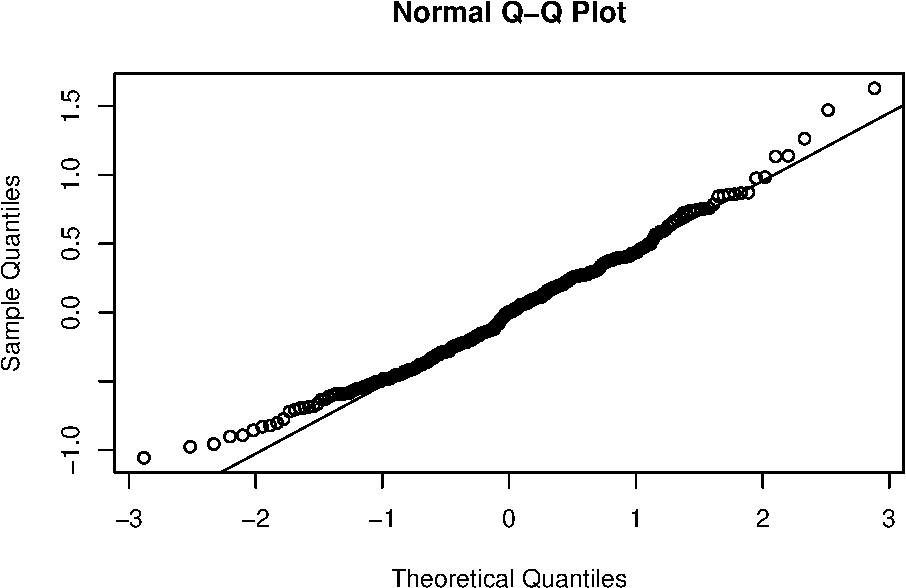
\includegraphics{A4_files/figure-latex/unnamed-chunk-33-1.pdf}

\vspace{0.3cm}

Se observa que la mayoría de los residuos se aproximan a la recta, por
lo que no se ve un comportamiento que vaya en contra del supuesto de
normalidad. Sin embargo, se procede al test de Shapiro-Wilk para
confirmarlo.

\vspace{0.3cm}

\begin{Shaded}
\begin{Highlighting}[]
\FunctionTok{shapiro.test}\NormalTok{(linear\_residuals)}
\end{Highlighting}
\end{Shaded}

\begin{verbatim}
## 
##  Shapiro-Wilk normality test
## 
## data:  linear_residuals
## W = 0.9869, p-value = 0.02071
\end{verbatim}

\vspace{0.3cm}

Como el \emph{p\_value} del test de Shapiro-Wilk es menor que el nivel
de significancia del 5\%, se rechaza la hipótesis nula y se acepta la
hipótesis alternativa. En este caso, se tiene que la variable aleatoria
que representa los errores del modelo no sigue una distribución normal.

\vspace{0.3cm}

\hypertarget{homocedasticidad-homogeneidad-de-varianzas}{%
\subsection{7.2 Homocedasticidad: Homogeneidad de
varianzas}\label{homocedasticidad-homogeneidad-de-varianzas}}

Otra de las condiciones de aplicación de ANOVA es la igualdad de
varianzas (homoscedasticidad). Aplicar un test para validar si los
grupos presentan igual varianza. Aplicad el test adecuado e interpretar
el resultado.

Nota: podéis usar tests como el de Levene o Bartlett test.

\vspace{0.3cm}

\begin{Shaded}
\begin{Highlighting}[]
\FunctionTok{bartlett.test}\NormalTok{(AE }\SpecialCharTok{\textasciitilde{}}\NormalTok{ Tipo, }\AttributeTok{data =}\NormalTok{ df)}
\end{Highlighting}
\end{Shaded}

\begin{verbatim}
## 
##  Bartlett test of homogeneity of variances
## 
## data:  AE by Tipo
## Bartlett's K-squared = 3.2658, df = 5, p-value = 0.6591
\end{verbatim}

\vspace{0.3cm}

Como el \emph{p\_value} es mayor que el nivel de significancia del 5\%,
aceptamos la hipótesis nula de que las varianzas son iguales.

\vspace{0.3cm}

\hypertarget{hipuxf3tesis-nula-y-alternativa}{%
\subsection{7.3 Hipótesis nula y
alternativa}\label{hipuxf3tesis-nula-y-alternativa}}

Independientemente de los resultados sobre la normalidad e
homoscedasticidad de los datos, proseguiremos con la aplicación del
análisis de varianza. Concretamente, se aplicará ANOVA de un factor
(one-way ANOVA o independent samples ANOVA) para investigar si existen
diferencias en el nivel de aire expulsado (AE) entre los distintos tipos
de fumadores. Escribid la hipótesis nula y alternativa.

\vspace{0.3cm}

\[ H_0: \mu_{NF} = \mu_{FP} = \mu_{NI} = \mu_{FL} = \mu_{FM} = \mu_{FI} = \mu \]
\[ H_1: \exists\mu_j \neq \mu, \ j=\{NF, FP, NI, FL, FM, FI\}\]

\vspace{0.3cm}

\hypertarget{cuxe1lculo-anova}{%
\subsection{7.4 Cálculo ANOVA}\label{cuxe1lculo-anova}}

Podéis usar la función aov.

\vspace{0.3cm}

\begin{Shaded}
\begin{Highlighting}[]
\NormalTok{anova\_model }\OtherTok{\textless{}{-}} \FunctionTok{aov}\NormalTok{(AE }\SpecialCharTok{\textasciitilde{}}\NormalTok{ Tipo, }\AttributeTok{data =}\NormalTok{ df)}
\NormalTok{summarized\_model }\OtherTok{\textless{}{-}} \FunctionTok{summary}\NormalTok{(anova\_model)}
\NormalTok{summarized\_model}
\end{Highlighting}
\end{Shaded}

\begin{verbatim}
##              Df Sum Sq Mean Sq F value   Pr(>F)    
## Tipo          5  20.86   4.171   17.88 4.03e-15 ***
## Residuals   247  57.63   0.233                     
## ---
## Signif. codes:  0 '***' 0.001 '**' 0.01 '*' 0.05 '.' 0.1 ' ' 1
\end{verbatim}

\newpage

\hypertarget{interpretaciuxf3n-2}{%
\subsection{7.5 Interpretación}\label{interpretaciuxf3n-2}}

Interpretad los resultados de la prueba ANOVA y relacionarlos con el
resultado gráfico del boxplot mostrado en el apartado 2.3.

\vspace{0.3cm}

Dado que el \emph{p\_value} es mucho más pequeño que el nivel de
significancia del 5\%, se puede rechazar la hipótesis nula y aceptar la
hipótesis alternativa. Esto es, que hay al menos un valor de la variable
\emph{Tipo} cuya media no es igual a las demás. Por tanto, \emph{Tipo}
es un factor significativo en el modelo para predecir \emph{AE}.

\vspace{0.3cm}

\hypertarget{profundizaciuxf3n-en-anova}{%
\subsection{7.6 Profundización en
ANOVA}\label{profundizaciuxf3n-en-anova}}

A partir de los resultados del modelo devuelto por aov, identificar las
variables SST (Total Sum of Squares), SSW (Within Sum of Squares), SSB
(Between Sum of Squares) y los grados de libertad. A partir de estos
valores, calcular manualmente el valor F, el valor crítico (a un nivel
de confianza del 95\%), y el valor p.~Interpretar los resultados y
explicar el significado de las variables SST, SSW y SSB.

\vspace{0.3cm}

Se obtiene la información a partir de la tabla de anova.

\vspace{0.3cm}

\begin{Shaded}
\begin{Highlighting}[]
\CommentTok{\# Se obtienen los Sum Squares}
\NormalTok{SS }\OtherTok{\textless{}{-}}\NormalTok{ summarized\_model[[}\DecValTok{1}\NormalTok{]]}\SpecialCharTok{$}\StringTok{"Sum Sq"}

\CommentTok{\# Primer elemento SSA, segundo SSE}
\NormalTok{SSB }\OtherTok{\textless{}{-}}\NormalTok{ SS[}\DecValTok{1}\NormalTok{]}
\NormalTok{SSW }\OtherTok{\textless{}{-}}\NormalTok{ SS[}\DecValTok{2}\NormalTok{]}
\NormalTok{SST }\OtherTok{\textless{}{-}}\NormalTok{ SSB }\SpecialCharTok{+}\NormalTok{ SSW}

\CommentTok{\# Obtener los grados de libertad}
\NormalTok{DFs }\OtherTok{\textless{}{-}}\NormalTok{ summarized\_model[[}\DecValTok{1}\NormalTok{]]}\SpecialCharTok{$}\NormalTok{Df}
\NormalTok{df.SSB }\OtherTok{\textless{}{-}}\NormalTok{ DFs[}\DecValTok{1}\NormalTok{]}
\NormalTok{df.SSW }\OtherTok{\textless{}{-}}\NormalTok{ DFs[}\DecValTok{2}\NormalTok{]}
\end{Highlighting}
\end{Shaded}

\vspace{0.3cm}

\hypertarget{cuxe1lculo-del-f-value}{%
\subsubsection{Cálculo del F value}\label{cuxe1lculo-del-f-value}}

\vspace{0.3cm}

\begin{Shaded}
\begin{Highlighting}[]
\NormalTok{F }\OtherTok{\textless{}{-}}\NormalTok{ (SSB}\SpecialCharTok{/}\NormalTok{df.SSB)}\SpecialCharTok{/}\NormalTok{(SSW}\SpecialCharTok{/}\NormalTok{df.SSW)}
\FunctionTok{cat}\NormalTok{(}\StringTok{"F value: "}\NormalTok{, F)}
\end{Highlighting}
\end{Shaded}

\begin{verbatim}
## F value:  17.87744
\end{verbatim}

\vspace{0.3cm}

\hypertarget{cuxe1lculo-del-valor-cruxedtico}{%
\subsubsection{Cálculo del Valor
crítico}\label{cuxe1lculo-del-valor-cruxedtico}}

\vspace{0.3cm}

\begin{Shaded}
\begin{Highlighting}[]
\NormalTok{critical }\OtherTok{\textless{}{-}} \FunctionTok{qf}\NormalTok{(}\AttributeTok{p =} \FloatTok{0.05}\NormalTok{, }\AttributeTok{df1 =}\NormalTok{ df.SSB, }\AttributeTok{df2 =}\NormalTok{ df.SSW, }\AttributeTok{lower.tail =} \ConstantTok{FALSE}\NormalTok{)}
\FunctionTok{cat}\NormalTok{(}\StringTok{"Critical value: "}\NormalTok{, critical)}
\end{Highlighting}
\end{Shaded}

\begin{verbatim}
## Critical value:  2.250576
\end{verbatim}

\newpage

\hypertarget{cuxe1lculo-del-p-value}{%
\subsubsection{Cálculo del P value}\label{cuxe1lculo-del-p-value}}

\vspace{0.3cm}

\begin{Shaded}
\begin{Highlighting}[]
\NormalTok{p\_value }\OtherTok{\textless{}{-}} \FunctionTok{pf}\NormalTok{(}\AttributeTok{q =}\NormalTok{ F, }\AttributeTok{df1 =}\NormalTok{ df.SSB, }\AttributeTok{df2 =}\NormalTok{ df.SSW, }\AttributeTok{lower.tail =} \ConstantTok{FALSE}\NormalTok{)}
\FunctionTok{cat}\NormalTok{(}\StringTok{"P value: "}\NormalTok{, p\_value)}
\end{Highlighting}
\end{Shaded}

\begin{verbatim}
## P value:  4.025786e-15
\end{verbatim}

\vspace{0.3cm}

Los resultados obtenidos coinciden con la tabla de \emph{aov}. El
\emph{P value} es más pequeño que el \(\alpha\), por lo que se confirma
el rechazo a la hipótesis nula y se acepta la hipótesis alternativa
(apartado 7.3).

\vspace{0.3cm}

La variable SST es la suma de los errores cuadrados totales, como se
puede ver la suma de SSB y SSW. La variable SSW es lo mismo que SSE, que
muestra la suma de los errores cuadrados, mientras que la variable SSB
es lo mismo que SSA, que es la suma de los cuadrados de los
tratamientos.

\vspace{0.3cm}

\hypertarget{fuerza-de-la-relaciuxf3n}{%
\subsection{7.7 Fuerza de la relación}\label{fuerza-de-la-relaciuxf3n}}

Calcular la fuerza de la relación e interpretar el resultado.

\vspace{0.3cm}

\begin{Shaded}
\begin{Highlighting}[]
\NormalTok{R2 }\OtherTok{\textless{}{-}}\NormalTok{ SSB}\SpecialCharTok{/}\NormalTok{SST}
\NormalTok{R2}
\end{Highlighting}
\end{Shaded}

\begin{verbatim}
## [1] 0.2657271
\end{verbatim}

\vspace{0.3cm}

El coeficiente de determinación es la proporción de variación de la
variable \emph{AE} frente al predictor \emph{Tipo}, que para este caso
asciende a un 26.57\%.

\newpage

\hypertarget{comparaciones-muxfaltiples}{%
\section{8 Comparaciones múltiples}\label{comparaciones-muxfaltiples}}

\begin{center}\rule{0.5\linewidth}{0.5pt}\end{center}

\vspace{0.3cm}

Independientemente del resultado obtenido en el apartado anterior,
realizamos un test de comparación múltiple entre los grupos. Este test
se aplica cuando el test ANOVA devuelve rechazar la hipótesis nula de
igualdad de medias. Por tanto, procederemos como si el test ANOVA
hubiera dado como resultado el rechazo de la hipótesis nula.

\vspace{0.3cm}

\hypertarget{test-pairwise}{%
\subsection{8.1 Test pairwise}\label{test-pairwise}}

Calcular las comparaciones entre grupos sin ningún tipo de corrección.
Podéis usar la función pairwise.t.test. Interpretar los resultados.

\vspace{0.3cm}

\begin{Shaded}
\begin{Highlighting}[]
\FunctionTok{pairwise.t.test}\NormalTok{(df}\SpecialCharTok{$}\NormalTok{AE, df}\SpecialCharTok{$}\NormalTok{Tipo, }\AttributeTok{p.adj =} \FunctionTok{c}\NormalTok{(}\StringTok{"none"}\NormalTok{))}
\end{Highlighting}
\end{Shaded}

\begin{verbatim}
## 
##  Pairwise comparisons using t tests with pooled SD 
## 
## data:  df$AE and df$Tipo 
## 
##    FI      FL      FM      FP      NF     
## FL 0.00165 -       -       -       -      
## FM 0.58175 0.00027 -       -       -      
## FP 0.00021 0.54864 2.9e-05 -       -      
## NF 5.4e-13 2.6e-05 2.6e-14 0.00035 -      
## NI 0.00011 0.46122 1.3e-05 0.89733 0.00048
## 
## P value adjustment method: none
\end{verbatim}

\vspace{0.3cm}

\begin{itemize}
\item
  Como podemos observar el valor del \emph{p\_value} que hemos obtenido
  para el par FM-FI es mayor que un nivel de significancia del 5\%, por
  lo que no tenemos evidencia estadística para rechazar la hipótesis de
  que ambos son similares.
\item
  Como podemos observar el valor del \emph{p\_value} que hemos obtenido
  para el par FP-FL es mayor que un nivel de significancia del 5\%, por
  lo que no tenemos evidencia estadística para rechazar la hipótesis de
  que ambos son similares.
\item
  Como podemos observar el valor del \emph{p\_value} que hemos obtenido
  para el par NI-FL es mayor que un nivel de significancia del 5\%, por
  lo que no tenemos evidencia estadística para rechazar la hipótesis de
  que ambos son similares.
\item
  Como podemos observar el valor del \emph{p\_value} que hemos obtenido
  para el par NI-FP es mayor que un nivel de significancia del 5\%, por
  lo que no tenemos evidencia estadística para rechazar la hipótesis de
  que ambos son similares.
\item
  Para todos los demás pares tenemos valores de \emph{p\_value} menores
  que un nivel de significancia del 5\%, por tanto se puede rechazar la
  hipótesis de que entre estas parejas se tiene una media similar. Esto
  nos indica que estos grupos son diferentes entre ellos.
\end{itemize}

\newpage

\hypertarget{correcciuxf3n-de-bonferroni}{%
\subsection{8.2 Corrección de
Bonferroni}\label{correcciuxf3n-de-bonferroni}}

Aplicar la corrección de Bonferroni en la comparación múltiple.
Interpretar el resultado y contrastar el resultado con el obtenido en el
test de comparaciones múltiples sin corrección.

\vspace{0.3cm}

\begin{Shaded}
\begin{Highlighting}[]
\FunctionTok{pairwise.t.test}\NormalTok{(df}\SpecialCharTok{$}\NormalTok{AE, df}\SpecialCharTok{$}\NormalTok{Tipo, }\AttributeTok{p.adj =} \FunctionTok{c}\NormalTok{(}\StringTok{"bonferroni"}\NormalTok{))}
\end{Highlighting}
\end{Shaded}

\begin{verbatim}
## 
##  Pairwise comparisons using t tests with pooled SD 
## 
## data:  df$AE and df$Tipo 
## 
##    FI      FL      FM      FP      NF     
## FL 0.02477 -       -       -       -      
## FM 1.00000 0.00409 -       -       -      
## FP 0.00315 1.00000 0.00043 -       -      
## NF 8.1e-12 0.00039 4.0e-13 0.00522 -      
## NI 0.00160 1.00000 0.00020 1.00000 0.00717
## 
## P value adjustment method: bonferroni
\end{verbatim}

\vspace{0.3cm}

Obtenemos los mismos resultados pero con valores más fáciles de
interpretar, que tienen más fortaleza a la hora de rechazar la
hipótesis.

\newpage

\hypertarget{anova-multifactorial}{%
\section{9 ANOVA multifactorial}\label{anova-multifactorial}}

\begin{center}\rule{0.5\linewidth}{0.5pt}\end{center}

\vspace{0.3cm}

En una segunda fase de la investigación se evalua el efecto del género
como variable independiente, además del efecto del tipo de fumador,
sobre la variable AE.

\vspace{0.3cm}

\hypertarget{anuxe1lisis-visual}{%
\subsection{9.1 Análisis visual}\label{anuxe1lisis-visual}}

\vspace{0.3cm}

Se realizará un primer estudio visual para determinar si existen efectos
principales o hay efectos de interacción entre género y tipo de fumador.
Para ello, seguir los pasos que se indican a continuación:

\vspace{0.3cm}

\begin{enumerate}
\def\labelenumi{\arabic{enumi}.}
\tightlist
\item
  Agrupar el conjunto de datos por tipo de fumador y género y calcular
  la media de AE en cada grupo. Podéis usar las instrucciones group\_by
  y summarise de la librería dplyr para realizar este proceso. Mostrar
  el conjunto de datos en forma de tabla, donde se muestre la media de
  cada grupo según el género y tipo de fumador.
\end{enumerate}

\vspace{0.3cm}

\begin{Shaded}
\begin{Highlighting}[]
\NormalTok{resumen }\OtherTok{\textless{}{-}}\NormalTok{ df }\SpecialCharTok{\%\textgreater{}\%}
    \FunctionTok{group\_by}\NormalTok{(genero, Tipo) }\SpecialCharTok{\%\textgreater{}\%}
    \FunctionTok{summarise}\NormalTok{(}\AttributeTok{means =} \FunctionTok{mean}\NormalTok{(AE), }\AttributeTok{counts =} \FunctionTok{length}\NormalTok{(AE))}
\NormalTok{resumen}
\end{Highlighting}
\end{Shaded}

\begin{verbatim}
## # A tibble: 12 x 4
## # Groups:   genero [2]
##    genero Tipo  means counts
##    <fct>  <fct> <dbl>  <int>
##  1 F      FI     1.27     24
##  2 F      FL     1.51     28
##  3 F      FM     1.07     22
##  4 F      FP     1.63     18
##  5 F      NF     1.93     29
##  6 F      NI     1.63     23
##  7 M      FI     1.14     17
##  8 M      FL     1.65     13
##  9 M      FM     1.27     17
## 10 M      FP     1.61     22
## 11 M      NF     2.07     21
## 12 M      NI     1.64     19
\end{verbatim}

\vspace{0.3cm}

\begin{enumerate}
\def\labelenumi{\arabic{enumi}.}
\setcounter{enumi}{1}
\tightlist
\item
  Mostrar en un gráfico el valor de AE medio para cada tipo de fumador y
  género. Podéis realizar este tipo de gráfico usando la función ggplot
  de la librería ggplot2.
\end{enumerate}

\vspace{0.3cm}

\begin{Shaded}
\begin{Highlighting}[]
\FunctionTok{ggplot}\NormalTok{(resumen, }\FunctionTok{aes}\NormalTok{(}\AttributeTok{fill =}\NormalTok{ genero, }\AttributeTok{x =}\NormalTok{ Tipo, }\AttributeTok{y =}\NormalTok{ means)) }\SpecialCharTok{+} \FunctionTok{geom\_bar}\NormalTok{(}\AttributeTok{position =} \StringTok{"dodge"}\NormalTok{,}
    \AttributeTok{stat =} \StringTok{"identity"}\NormalTok{) }\SpecialCharTok{+} \FunctionTok{scale\_color\_manual}\NormalTok{(}\AttributeTok{values =} \FunctionTok{c}\NormalTok{(}\StringTok{"\#0073C2FF"}\NormalTok{,}
    \StringTok{"\#EFC000FF"}\NormalTok{)) }\SpecialCharTok{+} \FunctionTok{scale\_fill\_manual}\NormalTok{(}\AttributeTok{values =} \FunctionTok{c}\NormalTok{(}\StringTok{"\#0073C2FF"}\NormalTok{,}
    \StringTok{"\#EFC000FF"}\NormalTok{)) }\SpecialCharTok{+} \FunctionTok{ylab}\NormalTok{(}\StringTok{"AE means"}\NormalTok{)}
\end{Highlighting}
\end{Shaded}

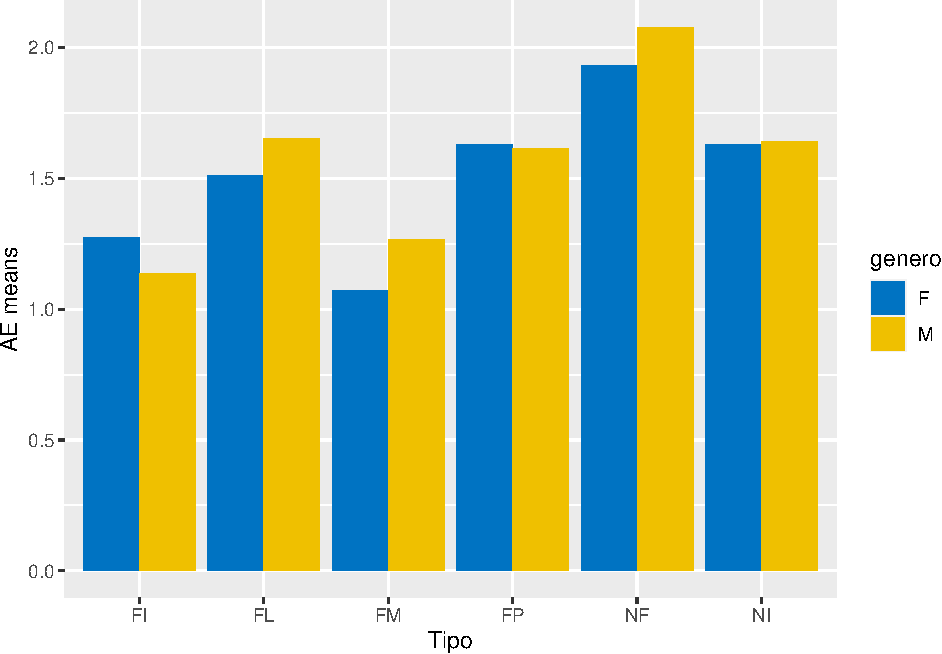
\includegraphics{A4_files/figure-latex/unnamed-chunk-45-1.pdf}

\vspace{0.3cm}

\begin{enumerate}
\def\labelenumi{\arabic{enumi}.}
\setcounter{enumi}{2}
\tightlist
\item
  Interpretar el resultado sobre si existen sólo efectos principales o
  existe interacción. Si existe interacción, explicar cómo se observa y
  qué efectos produce esta interacción.
\end{enumerate}

\vspace{0.3cm}

Para los valores NI y FP, la diferencia de la media de AE para el género
M y F no parece ser significativa. Sin embargo, sí puede verse en la
gráfica anterior que para valores como FI, FL, FM y NF puede existir una
diferencia considerable entre estas medias.

\vspace{0.3cm}

\hypertarget{anova-multifactorial-1}{%
\subsection{9.2 ANOVA multifactorial}\label{anova-multifactorial-1}}

Calcular ANOVA multifactorial para evaluar si la variable dependiente AE
se puede explicar a partir de las variables independientes género y tipo
de fumador. Incluid el efecto de la interacción.

\vspace{0.3cm}

\begin{Shaded}
\begin{Highlighting}[]
\NormalTok{multi\_anova }\OtherTok{\textless{}{-}} \FunctionTok{aov}\NormalTok{(AE }\SpecialCharTok{\textasciitilde{}}\NormalTok{ Tipo }\SpecialCharTok{*}\NormalTok{ genero, }\AttributeTok{data =}\NormalTok{ df)}
\FunctionTok{summary}\NormalTok{(multi\_anova)}
\end{Highlighting}
\end{Shaded}

\begin{verbatim}
##              Df Sum Sq Mean Sq F value   Pr(>F)    
## Tipo          5  20.86   4.171  17.739 5.81e-15 ***
## genero        1   0.20   0.197   0.838    0.361    
## Tipo:genero   5   0.76   0.153   0.650    0.661    
## Residuals   241  56.67   0.235                     
## ---
## Signif. codes:  0 '***' 0.001 '**' 0.01 '*' 0.05 '.' 0.1 ' ' 1
\end{verbatim}

\newpage

\hypertarget{interpretaciuxf3n-3}{%
\subsection{9.3 Interpretación}\label{interpretaciuxf3n-3}}

Interpretad el resultado.

\vspace{0.3cm}

A priori se puede decir que \emph{genero} no tiene evidencia estadística
suficiente para afirmar que es significativa para el modelo, eso ya que
el \emph{p\_value} es mayor que un nivel de significancia de 5\%. Esto
también le ocurre a la interacción. Por tanto, es mejor utilizar un
anota de un único factor en el que solamente se toma el \emph{Tipo}.

\newpage

\hypertarget{resumen-tuxe9cnico}{%
\section{10 Resumen técnico}\label{resumen-tuxe9cnico}}

\begin{center}\rule{0.5\linewidth}{0.5pt}\end{center}

\vspace{0.3cm}

Realizad una tabla con el resumen técnico de las preguntas de
investigación planteadas a lo largo de esta actividad.

\vspace{0.3cm}

\begin{longtable}[]{@{}
  >{\centering\arraybackslash}p{(\columnwidth - 4\tabcolsep) * \real{0.0638}}
  >{\centering\arraybackslash}p{(\columnwidth - 4\tabcolsep) * \real{0.3404}}
  >{\centering\arraybackslash}p{(\columnwidth - 4\tabcolsep) * \real{0.5957}}@{}}
\toprule()
\begin{minipage}[b]{\linewidth}\centering
N
\end{minipage} & \begin{minipage}[b]{\linewidth}\centering
Pregunta
\end{minipage} & \begin{minipage}[b]{\linewidth}\centering
Resultado y conclusión
\end{minipage} \\
\midrule()
\endhead
1 & ¿Se observan diferencias en la capacidad pulmonar en relación al
género? Interpretación desde gráficas. & Las distribuciones parecen
centradas en la media del intervalo {[}0;3{]}, aunque sí existen más
casos atípicos cuando el género es F. \\
--- & -------------- & -------------------------- \\
2 & ¿Se observan diferencias significativas entre los intervalos de
confianza de la capacidad pulmonar de mujeres y hombres? & Ambos
intervalos son relativamente similares puesto que varían recién en la
segunda cifra decimal,ambos rondan el 1.55 como valor central. \\
--- & -------------- & -------------------------- \\
3 & ¿Se observan diferencias significativas en la capacidad pulmonar de
mujeres y hombres? Interpretación a través de contraste de hipótesis. &
Como el \emph{p\_value} es mayor que el nivel de significancia, se debe
aceptar la hipótesis nula porque nohay evidencia suficiente para poder
descartarla. Por lo tanto, lo único que se puede decir es que la
capacidad pulmonar de ambos grupos se muestra igual. \\
--- & -------------- & -------------------------- \\
4 & ¿Podemos afirmar que la capacidad pulmonar de los fumadores es
inferior a la de no fumadores? & Ya que el \emph{p\_value} tiene un
valor menor al nivel de significancia, se puede rechazar la hipótesis
nula y aceptar la hipótesis alternativa. Por lo tanto, se tiene
evidencia estadística suficiente para inferir que la capacidad pulmonar
de los fumadores es menor que la de los no fumadores. \\
--- & -------------- & -------------------------- \\
5 & ¿Existen diferencias entre la capacidad pulmonar (AE) entre los
distintos tipos de fumadores/no fumadores? Si existen diferencias,
¿entre qué grupos están estas diferencias? & Dado que el \emph{p\_value}
es mucho más pequeño que el nivel de significancia del 5\%, se puede
rechazar la hipótesis nula y aceptar la hipótesis alternativa. Esto es,
que hay al menos un valor de la variable \emph{Tipo} cuya media no es
igual a las demás. Por tanto, \emph{Tipo} es un factor significativo en
el modelo para predecir \emph{AE}. La diferencia está en los pares
FL-FI, FP-FI, NF-FI, NI-FI, FM-FL, NF-FL, FP-FM, NF-FM, NI-FM, NF-FP,
NI-NF. \\
--- & -------------- & -------------------------- \\
\bottomrule()
\end{longtable}

\newpage

\hypertarget{resumen-ejecutivo}{%
\section{11 Resumen ejecutivo}\label{resumen-ejecutivo}}

\begin{center}\rule{0.5\linewidth}{0.5pt}\end{center}

\vspace{0.3cm}

Escribid un resumen ejecutivo como si tuvieráis que comunicar a una
audiencia no técnica. Por ejemplo, podría ser un equipo de gestores o
decisores, a los cuales se les debe informar sobre las consecuencias de
fumar sobre la capacidad pulmonar, para que puedan tomar las decisiones
necesarias.

\vspace{0.3cm}

A partir de toda la información obtenida durante la realización de este
informe, puede resumirse brevemente destacando la vinculación que existe
entre el tipo de fumador y la capacidad pulmonar de los individuos.
Incluso se puede ir un poco más allá pudiendo resaltar la estrecha
relación entre los tipos específicos de individuo con la capacidad
pulmonar.

\vspace{0.3cm}

La capacidad pulmonar presenta los mayores valores de la serie para
aquellos individuos de la muestra que están clasificados como No Fumador
(NF), mientras que los más bajos están presentes en los individuos
clasificados como Fumador Moderado (FM) y Fumador Intensivo (FI), lo
cual es observable en un contexto real.

\vspace{0.3cm}

En cuanto a género se refiere, no se ha determinado un tipo de vínculo
que pueda dar lugar a una relación entre el género y la capacidad
pulmonar.

\end{document}
